%%**************************************************************
%% Vorlage fuer Bachelorarbeiten (o.ä.) der DHBW
%%
%% Autor: Tobias Dreher, Yves Fischer
%% Datum: 06.07.2011
%%**************************************************************

\newcommand{\pdftitel}{Test Framework für Unity}
\newcommand{\autor}{Lennart Hensler}
\newcommand{\arbeit}{Studienarbeit}

%
% Nahezu alle Einstellungen koennen hier getaetigt werden
%

\documentclass[%
	pdftex,
	oneside,		% Einseitiger Druck.
	12pt,			% Schriftgroesse
	parskip=half,	% Halbe Zeile Abstand zwischen Absätzen.
	headsepline,	% Linie nach Kopfzeile.
	footsepline,	% Linie vor Fusszeile.
	abstracton,	    % Abstract Überschriften
	ngerman,		% Translator
]{scrreprt}

%Seitengroesse
\usepackage{fullpage}

%Zeilenumbruch und mehr
\usepackage[activate]{microtype}

% Zeichencodierung
\usepackage[utf8]{inputenc}
\usepackage[T1]{fontenc}

% Zeilenabstand
\usepackage[onehalfspacing]{setspace}

% Index-Erstellung
\usepackage{makeidx}

% Lokalisierung (neue deutsche Rechtschreibung)
\usepackage[ngerman]{babel}

% Anführungszeichen 
\usepackage[babel,german=quotes]{csquotes}
%\usepackage[style=swiss]{csquotes}


% Spezielle Tabellenform fuer Deckblatt
\usepackage{longtable}
\setlength{\tabcolsep}{10pt} %Abstand zwischen Spalten
\renewcommand{\arraystretch}{1.5} %Zeilenabstand

% Grafiken
\usepackage{graphicx}

% Mathematische Textsaetze
%\usepackage{amsmath}
%\usepackage{amssymb}

% Pakete um Textteile drehen zu können, oder eine Seite Querformat anzeigen kann.
%\usepackage{rotating}
%\usepackage{lscape}

% Farben
\usepackage{color}
\definecolor{LinkColor}{rgb}{0,0,0.2}
\definecolor{ListingBackground}{rgb}{0.92,0.92,0.92}
\definecolor{ListingKeyword}{RGB}{57, 135, 214}
\definecolor{ListingString}{RGB}{214, 136, 82}
\definecolor{ListingComment}{RGB}{84, 139, 61}

% PDF Einstellungen
%\usepackage[%
%	pdftitle={\pdftitel},
%	pdfauthor={\autor},
%	pdfsubject={\arbeit},
%	pdfcreator={pdflatex, LaTeX with KOMA-Script},
%	pdfpagemode=UseOutlines, % Beim Oeffnen Inhaltsverzeichnis anzeigen
%	pdfdisplaydoctitle=true, % Dokumenttitel statt Dateiname anzeigen.
%	pdflang=de % Sprache des Dokuments.
%]{hyperref}

% (Farb-)einstellungen für die Links im PDF
%\hypersetup{%
%	colorlinks=false, % Aktivieren von farbigen Links im Dokument
%	linkcolor=LinkColor, % Farbe festlegen
%	citecolor=LinkColor,
%	filecolor=LinkColor,
%	menucolor=LinkColor,
%	urlcolor=LinkColor,
%	bookmarksnumbered=true % Überschriftsnummerierung im PDF Inhalt anzeigen.
%}
\usepackage{hyperref}

% Verschiedene Schriftarten
%\usepackage{goudysans}
%\usepackage{lmodern}
%\usepackage{libertine}
\usepackage{palatino} 

% Hurenkinder und Schusterjungen verhindern
% http://projekte.dante.de/DanteFAQ/Silbentrennung
\clubpenalty=10000
\widowpenalty=10000
\displaywidowpenalty=10000

% Quellcode
\usepackage{listings}
\renewcommand{\lstlistingname}{Code} %Changing the label of listings
\renewcommand{\lstlistlistingname}{Codeverzeichnis} %Changing the name of the listings list
\lstloadlanguages{[Sharp]C}
\lstset{%
	language=[Sharp]C,		 % Sprache des Quellcodes
	numbers=left,            % Zelennummern links
	stepnumber=1,            % Jede Zeile nummerieren.
	numbersep=5pt,           % 5pt Abstand zum Quellcode
	numberstyle=\scriptsize, % Zeichengrösse 'tiny' für die Nummern.
	frame=lines,			 % Linie oben und unten als Rahmen
	breaklines=true,         % Zeilen umbrechen wenn notwendig.
	breakautoindent=true,    % Nach dem Zeilenumbruch Zeile einrücken.
	postbreak=\space,        % Bei Leerzeichen umbrechen.
	tabsize=2,               % Tabulatorgrösse 2
	showspaces=false,        % Leerzeichen nicht anzeigen.
	showstringspaces=false,  % Leerzeichen auch in Strings ('') nicht anzeigen.
	extendedchars=true,      % Alle Zeichen vom Latin1 Zeichensatz anzeigen.
	captionpos=b,            % sets the caption-position to bottom
	backgroundcolor=\color{ListingBackground}, % Hintergrundfarbe des Quellcodes setzen.
	basicstyle=\ttfamily\footnotesize,			  % Nichtproportionale Schrift, klein für den Quellcode
	keywordstyle=\bfseries\color{ListingKeyword}, % Keywords fett und blau
	commentstyle=\color{ListingComment},		  % Kommentare grün
	stringstyle=\color{ListingString}			  % Strings orange
}

% Glossar
\usepackage[
	nonumberlist, %keine Seitenzahlen anzeigen
	acronym,      %ein Abkürzungsverzeichnis erstellen
	%section,     %im Inhaltsverzeichnis auf section-Ebene erscheinen
	toc,          %Einträge im Inhaltsverzeichnis
]{glossaries}

% Fussnoten
\usepackage[perpage, hang, multiple, stable]{footmisc}

% Text Bilder umfließen lassen
\usepackage{wrapfig}

% Captions von Bildern
\usepackage[margin=10pt,format=hang,indention=-1.5cm,singlelinecheck=false,font=small,labelfont=bf]{caption}
\usepackage{subcaption}

% Appendix
\usepackage{appendix}

% geschachtelte Aufzählungen
\usepackage{enumitem}

% Titel, Autor und Datum
\title{\titel}
\author{\autor}
\date{\datum}

%Weitere Kommandos
\newcommand{\TODO}[1]{\textcolor{red}{\textbf{TODO:} #1}} 

% Ab jetzt können auch Umlaute verwendet werden
\newcommand{\titel}{Test Framework für Unity}
\newcommand{\martrikelnr}{3581041}
\newcommand{\kurs}{TAI10B1}
\newcommand{\datumAbgabe}{27. Mai 2013}
\newcommand{\firma}{}
\newcommand{\firmenort}{}
\newcommand{\abgabeort}{Karlsruhe}
\newcommand{\abschluss}{Bachelor of Science}
\newcommand{\studiengang}{Studienganges Angewandte Informatik}
\newcommand{\dhbw}{Karlsruhe}
\newcommand{\betreuer}{Daniel Lindner}
\newcommand{\gutachter}{}
\newcommand{\zeitraum}{}

\makeglossaries
\input{glossary}

\begin{document}

	% Deckblatt
	\begin{spacing}{1}
		\input{deckblatt}
	\end{spacing}
	\newpage

	\renewcommand{\thepage}{\Roman{page}}
	\setcounter{page}{1}

	% Erklärung
	\input{erklaerung}
	\newpage

	% Abstract
	\pagestyle{empty}

\renewcommand{\abstractname}{Zusammenfassung}
\begin{abstract}
Diese Studienarbeit handelt von der Entwicklung eines Frameworks automatisierter Tests für die Spiele-Engine Unity. Im Rahmen einer vorherigen Studienarbeit wurde versucht ein Spiel testgetrieben zu entwickeln. Dabei hat sich herausgestellt, dass die verhaltenssteuernden Komponenten eines Spiels nur marginal testen lassen, ohne die Art zu entwickeln stark an eine mögliche Testbarkeit anzupassen. Aus diesem Grund möchte ich versuchen ein eigenes Framework zu entwickeln, welches einem mehr Möglichkeiten bietet. Als erstes Stelle ich die verschiedenen Arten von Tests vor. Als nächstes analysiere ich die schon vorhanden Frameworks und beschreibe einen möglichen Erstentwurf. Zum Schluss wird die konkrete Implementierung vorgestellt und ich gebe einen Ausblick auf die weiteren Entwicklungsmöglichkeiten.
\end{abstract}


\renewcommand{\abstractname}{Summary}
\begin{abstract}
This seminar paper is about the development of a test framework for the game engine Unity. In the context of a previous seminar paper had been tested, how to develop a game test driven. It turned out, that it's hard to test the compoments that define the behaviour of a game, without adapting the development for testability. For this reason I want to develop my own framework, which has more possibilites. At first I'll explain the different types of tests. Then I analyse the existing test frameworks and discribe a first design for my framework. Finally I present the concrete implementation and I give an outlook for future features.
\end{abstract}

	\newpage

	\pagestyle{plain}

	% Inhaltsverzeichnis
	\begin{spacing}{1.1}
		\setcounter{tocdepth}{1}
		\tableofcontents
	\end{spacing}
	\newpage

	\renewcommand{\thepage}{\arabic{page}}
	\setcounter{page}{1}
	
	% Inhalt
	\chapter{Einleitung}



\section{Test Driven Development}

Die testgetriebene Entwicklung (im englischen \textit{test-driven development} oder kurz TDD, wird auch \textit{test first development} genannt) ist ein Teil der agilen Softwareentwicklung und basiert darauf, dass die Tests vor dem Produktivcode geschrieben werden. Da Diese dabei eine zentrale Rolle spielen, geben wir zunächst einen Überblick über die unterschiedlichen Arten. Im Anschluss gehen wir detaillierter auf die testgetriebene Entwicklung ein.

\subsection{Arten von Tests}

Tests sollen einen bestimmten Teil des Programms auf seine Korrektheit überprüfen und dabei möglichst schnell und automatisiert ablaufen. Je nachdem wie umfangreich der getestete Bereich ist und welche Kenntnisse der Test/Entwickler von der inneren Umsetzung des Programms hat, kann man die Tests kategorisieren.

\paragraph{White- und Black-Box-Tests} Die gröbste Einteilung ist die Unterscheidung zwischen White- und Black-Box-Tests. Dabei wird nicht der Umfang des getesteten Bereichs berücksichtigt, sondern lediglich ob der Entwickler des Tests Kenntnisse über die Implementierung der zu testenden Funktionen hat.\\
Bei White-Box-Tests ist dies der Fall. Idealerweise, sollte der Entwickler der den Produktivcode geschrieben hat auch den dazugehörigen Test implementieren. Mit dieser Art von Test werden die inneren Strukturen eines Programms überprüft. Also zum Beispiel, dass eine Methode nicht mit Parametern aufgerufen werden kann, die Fehler verursachen könnten. Hierbei wird nur getestet ob das Programm fehlerfrei abläuft und nicht ob die einzelnen Methoden das gewünschte Verhalten aufweisen.

Im Gegensatz dazu stehen die Black-Box-Tests, deren Entwickler keinerlei Kenntnisse über die Umsetzung haben sollte. Ansonsten könnten beim Schreiben der Tests Dinge implizit als erfüllt angesehen werden, die allerdings getestet werden müssen. Dadurch wäre es möglich, dass bei nachträglichen Änderungen Fehler auftreten, ohne dass ein Test fehlschlägt.\\
Black-Box-Tests sollen verifizieren, dass das Programm die Spezifikationen des Kunden erfüllt.

Diese beiden Testarten ergänzen sich gegenseitig und es sollten immer sowohl White-Box, als auch Black-Box-Tests erstellt werden, um das Produkt zu überprüfen und robust gegen Fehler bei nachträgliche Änderungen zu machen.\\
Schematische Darstellungen dieser Testarten sieht man in \autoref{fig:White_Box_Test} und \autoref{fig:Black_Box_Test} auf den nächsten Seiten.

\paragraph{Unit-Tests} sind die kleinsten Einheiten unter den Tests. Sie sollen die einzelnen Methoden einer Klasse auf einen fehlerfreien Ablauf und ein korrektes Verhalten hin testen. Dadurch kann man im Verlauf der Entwicklung Änderungen am Programm vornehmen, ohne dass die Funktionalitäten der Module unbemerkt zerstört werden (insofern die Tests eine ausreichende Abdeckung erreichen).\\
Die einzelnen Tests sollten unabhängig voneinander und auch von den anderen Komponenten sein. Falls Verbindungen zwischen den Komponenten bestehen, sollten diese durch \textit{Mock}-Objekte entkoppelt werden. Diese erben von der entsprechenden Klasse und überschreiben deren Methoden auf eine geeignete Art. Zum Beispiel könnten sie einfach leer gelassen werden, was man als \textit{Stub} bezeichnet. Oder sie geben einen festen Wert zurück. \textit{Mock}-Klassen können selbst erstellt werden und sind meistens innere Klassen der Testklasse, allerdings gibt es auch \textit{Mock}-Frameworks, welche generisch \textit{Mocks} für beliebige Klassen oder Interfaces erzeugen können. Das Verhalten der Methoden eines Mocks, lässt sich mit diesen zur Laufzeit festlegen. Zum Beispiel dass ein fester Wert zurückgeliefert wird, oder eine Exception geworfen werden soll.\\ Beispiele sind \textit{JMock} für Java oder \textit{Moq} für C\#.\\
Außerdem sollten Unit-Tests sehr schnell ablaufen (im Millisekunden-Bereich), um nach jeder Änderung durchgeführt werden zu können, ohne die Entwicklung aufzuhalten.

Eine schematische Darstellung von Unit-Tests sieht man in \autoref{fig:Unit_Test}.

\paragraph{Integrationstests} Die nächsthöhere Stufe von Tests sind Integrationstests. Diese testen das Zusammenspiel mehrere Komponenten, eventuell auch mit Systemressourcen, auf ihre Korrektheit. Einen Unit-Test kann man zu einem Integrationstest machen, indem man die \textit{Mock}-Objekte durch die im Produktivbetrieb verwendet Klassen ersetzt und die Bedingungen entsprechend anpasst.

Integrationstests dürfen länger dauern als Unit-Tests, sollten dennoch schnell durchgeführt werden können.

Eine schematische Darstellung von Integrationstests sieht man in \autoref{fig:Integration_Test}.\\\\\\\\\\

\begin{figure}[h]
\centering
\includegraphics[width=0.8\linewidth]{./images/Kapitel_Einleitung/White_Box_Test.pdf}
\caption[Schematische Darstellung eines White-Box-Tests]{Schematische Darstellung eines White-Box-Tests\\Der Entwickler sollte sich gut mit dem zu testenden Code auskennen. Der Test verifiziert, dass die Methode korrekt ausgeführt wird.}
\label{fig:White_Box_Test}
\end{figure}

\begin{figure}[h]
\centering
\includegraphics[width=0.8\linewidth]{./images/Kapitel_Einleitung/Black_Box_Test.pdf}
\caption[Schematische Darstellung eines Black-Box-Tests]{Schematische Darstellung eines Black-Box-Tests\\Öffentliche Klassen und Methoden, sowie deren Beschreibungen sind dem Entwickler bekannt. Die konkrete Implementierung allerdings ist nicht einsehbar. Der Test verifiziert das Verhalten der zu testenden Klasse.}
\label{fig:Black_Box_Test}
\end{figure}

\clearpage

\paragraph{Akzeptanztests} sollen die Korrektheit des Verhaltens eines ganzen Systems prüfen. Dabei soll er sowohl die Benutzerschnittstelle, als auch die einzelnen Komponenten und die Systemressourcen abdecken. Allerdings testen diese nicht die innere Struktur des Systems (sind also Black-Box-Tests), sondern sollen gewährleisten, dass ein System sich so verhält, wie es der Kunde im Lastenheft definiert hat. Idealerweise verwendet der Test dabei nur die Schnittstellen, die ein Kunde auch verwenden würde (z.B. über Eingaben auf der GUI), um möglichst nahe an ein natürliches Verhalten zu kommen.\\
Akzeptanztests können durchaus länger dauern, da sie das gesamte Verhalten eines Systems repräsentieren, welches nur nach größeren Veränderungen getestet werden muss.

\begin{figure}[h]
\centering
	\begin{subfigure}[b]{0.29\textwidth}
	\centering
	\captionsetup{justification=centering}
	\includegraphics[width=\textwidth]{./images/Kapitel_Einleitung/Unit_Test.png}
	\caption{Unit-Test}
	\label{fig:Unit_Test}
	\end{subfigure}
	\begin{subfigure}[b]{0.29\textwidth}
	\centering
	\captionsetup{justification=centering}
	\includegraphics[width=\textwidth]{./images/Kapitel_Einleitung/Integrations_Test.png}
	\caption{Integrationstest}
	\label{fig:Integration_Test}
	\end{subfigure}
	\begin{subfigure}[b]{0.39\textwidth}
	\centering
	\captionsetup{justification=centering}
	\includegraphics[width=\textwidth]{./images/Kapitel_Einleitung/Akzeptanz_Test.png}
	\caption{Akzeptanztest}
	\label{fig:Acceptance_Test}
	\end{subfigure}
\caption[Schematische Darstellung der unterschiedlichen Testarten]{Schematische Darstellung der unterschiedlichen Testarten\\(a) testet die einzelnen Methoden einer Komponente. Alle anderen benötigten Komponenten sollten als Mock-Objekte eingebunden werden.\\(b) testet das Verhalten mehrere Komponenten und eventuell im Zusammenhang mit Systemressourcen\\(c) testet einen Großteil der Komponenten eines Programms mit den Systemressourcen nach den Anforderungen des Kunden.\\
Quelle: \url{http://schneide.wordpress.com/2011/09/05/a-shot-at-definitions-beyond-unit-test/}}
\label{fig:UnitIntegrationAcceptanceTest_Comparison}
\end{figure}
\clearpage

\subsection{Grundsätze und Funktionsweise von TDD}

Die testgetriebene Entwicklung arbeitet nach dem an und für sich einfachen Prinzip, die Tests \textbf{vor} dem Produktivcode zu schreiben. Um TDD richtig anzuwenden, sollten ein paar Dinge beachtet werden. Dennoch überwiegen die daraus resultierenden Vorteile diesen Mehraufwand. In diesem Abschnitt erläutern wir welche das sind, wie der Ablauf von TDD ist und was es dabei zu beachten gilt. Dabei orientieren wir uns an dem Buch \textit{Growing Object-Oriented Software, Guided by Tests} \cite{FRE10}.

Bei der testgetriebenen Entwicklung schreibt man zunächst einen Unit-Test, der das Verhalten der zu testenden Komponente definiert. Da deren innere Struktur unbekannt ist, wird dieser automatisch als ein Black-Box-Test implementiert. Dieser muss anfangs fehlschlagen, da die Komponente noch nicht implementiert, beziehungsweise nicht vorhanden ist. Danach sollte man diese auf möglichst einfache Art und Weise implementieren, damit der Test erfolgreich ausgeführt wird. Dadurch vermeidet man überflüssigen Code. Anschließend sollte der Test erweitert werden um die Kontrolle über potentielle Fehler zu behalten (White-Box-Test). Das Resultat hat Eigenschaften beider Testarten und wird deswegen auch als \textit{Grey-Box-Test}\footnote{\url{http://de.wikipedia.org/wiki/Grey-Box-Test}} bezeichnet. Abschließend refactored man seinen Produktivcode, falls dies nötig sein sollte. Wann und wie man refactoren sollte wird später angesprochen. Für detailliertere Informationen verweisen wir auf \cite{FOW99}.\\
Dieser Vorgang wird solange wiederholt, bis alle benötigten Komponenten und Funktionen implementiert sind. Diesen Zyklus kann man mit identischen Zyklen für Integrations- und Akzeptanztests umschließt, sodass eine größere und realitätsnähere Testabdeckung entsteht.

Ein großer Vorteil von TDD ist, dass man automatisch jede Komponente mit Tests überwacht. Dies ist nicht der Fall, wenn man die Tests nach dem Produktivcode schreiben würde. Das liegt daran, dass die Tests meistens gegen Ende der Entwicklung geschrieben werden. Zu diesem Zeitpunkt ist der Druck auf die Entwickler allerdings am größten, weswegen im Zweifelsfall auf Tests verzichtet wird, da diese keine weiteren Funktionalitäten hervorbringen. Außerdem könnten die Komponenten zu einem so späten Zeitpunkt sehr stark miteinander verbunden sein, wodurch die einzelnen Tests groß und unübersichtlich werden. Sollten trotz alldem Tests entwickelt werden, müssen alle Funktionalitäten auf einmal getestet werden, was eine undankbare Aufgabe darstellt. TDD hat hier den Vorteil, dass Tests und Produktivcode abwechselnd Stück für Stück implementiert werden.\\
Ein weiterer positiver Aspekt von TDD ist, dass die Entwickler wesentlich schneller und öfter Feedback über ihr Programm erhalten. Dies ermöglicht einem die Qualität seines Produkts erheblich zu steigern, da man auf Fehler und Unstimmigkeiten mit den Kundenwünschen aufmerksam gemacht wird. Dies ist bei Spielen besonders wichtig, da es mit der Kundenzufriedenheit steht und fällt (besonders wenn man noch keine große Fangemeinde etablieren konnte).\\
TDD ermöglicht es einem, leichter wartbare und erweiterbare Systeme zu schreiben. Denn dadurch, dass die Funktionen eine nach der anderen implementiert werden, ist es modularer und es entstehen weniger Abhängigkeiten zwischen den einzelnen Komponenten (vor allem, wenn man konsequent Mock-Objekte verwendet). Wenn man zusätzlich noch viele Interfaces einsetzt, können neue Funktionalitäten leichter nachträglich hinzugefügt werden. Durch die breite Testabdeckung ist das System zudem robuster gegenüber Fehler durch Änderungen, wodurch man leichter refactoren und sorgenfreier entwickeln kann, da daraus resultierende Defekte sofort erkannt werden.\\
Dadurch, dass die Tests geschrieben werden ohne dass man Kenntnis darüber hat wie die innere Struktur aussieht, entsteht besser lesbarer Code. Man hat nur die Vorgabe was der Zweck der aktuellen Komponente sein soll und kann die Methoden entsprechend benennen. Es hilft einem auch, zu entscheiden, welche Methoden von außen sichtbar sein sollen und welche nur der konkreten Implementierung bekannt sein müssen. Dadurch erhält man wesentlich schlankere und übersichtlichere Schnittstellen.\\
Ließen sich diese Vorteile für die Spielentwicklung einsetzen, würde dies einen erheblichen Fortschritt darstellen.

Um die oben aufgeführten Vorteile zu erhalten, sollte - außer dass man die Tests vor dem Produktivcode schreibt - noch einiges beachtet werden. Steve Freeman und Nat Pryce haben in \cite[Seite 6]{FRE10} eine goldene Regel des TDD aufgestellt:

\begin{quotation}
\textbf{\textit{\grqq Never write new functionality without a failing test.\grqq}}
\end{quotation}

Dies soll verhindern, dass der TDD-Zyklus nicht unterbrochen wird und dadurch manche Codeabschnitte ungetestet bleiben. Außerdem hilft es einem keine unnötigen Funktionen einzubauen, die vom Kunden nicht gewünscht sind. Denn die Tests orientieren sich an den Vorgaben des Kunden und solange man die Tests immer zuerst schreibt, wird auch nur diese Funktionalität entwickelt.\\
Als äußerst wichtig werden auch Akzeptanztests angesehen, die das Verhalten eines realen Anwenders möglichst genau simulieren. Sie sollen nur über die definierten Schnittstellen mit dem System kommunizieren, ohne die interne Implementierung direkt aufzurufen. Solche Tests bezeichnen sie als \textit{End-To-End-Tests} und sollen das System so testen, wie es an den Kunden ausgeliefert werden soll. Dazu gehört, dass die Unit-Tests durchlaufen werden, die benötigten Pakete eingebunden werden, das System in einer produktiv-ähnlichen Umgebung gebaut wird und die Akzeptanztests ausgeführt werden. Diese Art des Testens stellt einen erheblichen Aufwand dar, allerdings kann man erst dadurch sagen, dass das System auch beim Kunden fehlerfrei funktioniert.

Bevor man mit der testgetriebenen Entwicklung produktiv werden kann, muss man ein Grundgerüst für das Projekt bauen. Dieses wird als \textit{laufendes Skelette} \cite[orig. \textit{walking Skeleton}, Seite 32]{FRE10} bezeichnet und stellt die kleinste mögliche Implementierung einer Funktionalität dar, welche sich automatisch bauen lässt und worüber man einen End-To-End-Test schreiben kann \cite{COC04}. Für das Grundgerüst benötigt man einen kleinen Erstentwurf der Programmstruktur. Dieser soll noch keine konkreten Methoden oder Attribute enthalten, sondern nur darstellen welche Komponenten voraussichtlich gebraucht werden und wie diese miteinander kommunizieren. Hierbei orientiert man sich am besten an den Kundenanforderungen.\\
Dadurch, dass zu Beginn die konkrete Struktur unklar ist, ist das Schreiben von Tests am Anfang aufwendiger und chaotisch. Des weiteren kann es zu vielen nachträglichen Änderungen kommen, da man während der Entwicklung neue Erkenntnisse gewinnt. Allerdings ist das Ende des Projekts wesentlich kontrollierter, da man bereits eine solide Testbasis hat, welche einem Gewissheit gibt, dass das System so funktioniert wie es soll. Schreibt man die Tests am Ende, hat man das Problem sowohl diese, als auch die auf der Strecke gebliebenen Funktionen zu implementieren. Die testgetriebene Entwicklung verlagert den stressigen Teil des Projekts an den Anfang, wobei man zu diesem Zeitpunkt besser auf die auftretenden Probleme eingehen kann, anstatt kurze Zeit vor dem Veröffentlichungstermin.

Um den Zyklus der testgetriebenen Entwicklung am Laufen zu halten, gilt es weitere Dinge zu beachten, welche in \cite{FRE10} ab Seite 39 ausführlich beschrieben werden. Die wichtigsten Verhaltensregeln stellen wir hier nun kurz vor:

\begin{description}
\item[\small Jede neue Funktionalität soll mit einem Black-Box-Test beginnen]~\\
	Dadurch definiert man das Verhalten, ohne die innere Struktur zu berücksichtigen und erhält schlanke Schnittstellen. Die konkrete Implementierung kann sich nun laufend ändern und man hat dennoch einen Test der sicherstellt, dass das Verhalten korrekt ist.
\item[\small Unterscheiden zwischen fortschrittsmessenden und Rückschritt erkennenenden Tests]
	Neue Akzeptanztests stellen eine noch nicht implementierte Funktion dar. Sobald sie fehlerfrei ausgeführt werden, ist die Funktion fertig. Sie messen demnach den Fortschritt des Projekts.\\
	Sobald ein Akzeptanztest implementiert wurd,e misst er keinen Fortschritt mehr, sondern stellt sicher dass die Funktion fehlerfrei bleibt. Schlägt ein Test fehl, hat er einen Rückschritt erkannt.
\item[\small Tests sollen wohlformuliert sein]~\\
	Die Tests sollen das Verhalten, welches sie testen, möglichst genau beschreiben, sodass man auch bei späterem Betrachten weiß, was getestet wird. Schlägt der Test fehl, sollte eine aussagekräftige Fehlermeldung ausgegeben werden.
\item[\small Tests zuerst fehlschlagen lassen]~\\
	Nachdem man einen Test geschrieben hat, soll man diesen immer zuerst fehlschlagen lassen, bevor man den Produktivcode dazu schreibt. Dadurch erkennt man, ob einen die Fehlermeldung an die richtige Stelle leitet. Dadurch lässt sich ein später auftretender Fehler leichter beheben. Außerdem erkennt man Design-Fehler, falls der Test in einer anderen Weise als erwartet fehlschlägt.
\item[\small Teste das Verhalten, nicht die Methoden]~\\
	Es ist wichtiger ein korrektes Verhalten zu testen und nicht die einzelnen Zeilen jeder Methode. Auch eine hundertprozentige Testabdeckung garantiert kein fehlerfreies System. Tests sollten so formuliert werden, dass sie aussagen was sie testen und nicht welche Methode.
\item[\small Man soll auf seine Tests hören]~\\
	Wenn man auf eine schwierig zu testende Stelle trifft, sollte man sich nicht fragen, wie man diese testen kann, sondern warum es schwer ist sie zu testen. Dies ist meistens ein Anzeichen dafür, dass die Struktur refactored werden muss. Denn wenn etwas schwierig zu testen ist, ist es meist auch schwer zu ändern oder zu erweitern. Dies fällt allerdings meist erst später auf, weswegen man das Problem lösen sollte, solange es noch \grqq frisch\grqq~ist.
\end{description}

Da Refactoring ein wesentlicher Bestandteil der testgetriebenen Entwicklung ist, steht in \cite{FRE10} wann man refactoren sollte und wie man am besten mit den Tests verfährt. Wichtig ist, dass Refactoring keinen Geschwindigkeits- oder Funktionsvorteil bringt, sondern nur besser Wartbarkeit und Lesbarkeit. Die Hinweise beziehen sich meist darauf, dass nur die benötigten Teile einer Komponente nach außen sichtbar sein sollen und der Rest geheim bleibt. Außerdem helfen sie die einzelnen Komponenten richtig zu strukturieren, indem große gespalten werden und häufig auftretende Gruppen von Merkmalen zu einer neuen Komponente zusammengefasst werden. Auch hier wollen wir die wichtigsten Tipps vorstellen:

\begin{description}
\item[\small Teilen großer Komponenten]~\\
	Wenn eine Komponente während der Entwicklung sehr groß wird, kann man sie meistens in kleinere Komponenten unterteilen, welche anschließend separat getestet werden. Dadurch erhält man eine modulare Struktur und kleinere, übersichtlichere Tests. Außerdem werden einem die Abhängigkeiten seines Programms vor Augen geführt.
\item[\small Definieren eines neuen Services]~\\
	Wenn man den einzelnen Komponenten immer weitere Verhalten zuweist, kann es sein, dass diese nicht in die Komponente gehören. In diesem Fall sollten die Verhalten in einen neuen Service ausgelagert werden.\\
	Dafür wird dieser zunächst (zum Beispiel in Form eines Interfaces) definiert und im Unit-Test der Komponente gemocked. Anschließend werden Tests für diese Komponenten geschrieben.
\item[\small Bündelung von Komponenten]~\\
	Falls man eine Menge zusammenhängender Komponenten findet, kann man diese zu einer neuen Komponente vereinen. Diese verringert die Komplexität, da nur die relevanten Teile nach außen sichtbar sind. Dadurch wird die Domain besser verständlich und die Tests werden übersichtlicher, da man die neue Komponente separat testen kann.
\end{description}

Hält man sich an alle genannten Verhaltensregeln, bekommt man ein leichter wartbares und verständliches System mit den oben aufgeführten Vorteilen. Allerdings muss man sich an die Art der testgetriebenen Entwicklung erst gewöhnen, sollte diszipliniert sein und seine Erfahrung damit machen, bevor man damit souverän entwickeln kann.
\pagebreak

\section{Unity 3D}

\textit{Unity 3D} (mittlerweile nur noch \textit{Unity}) ist eine Spiele-Engine, welche für viele verschiedene Anwendungen, wie Spiele, Lernsoftware, sowie 3D-Animationsfilme verwendet wird. Der Hersteller bezeichnet die Software selber als \textit{Spieleentwicklungs-Ökosystem}\footnote{Zu lesen unter \url{http://unity3d.com/unity/}}, da sie neben der Engine selber eine komplette Entwicklungsumgebung für Spiele bietet.\\
Die Umgebung erlaubt es einem, die Spiele auch auf andere Plattformen zu portieren, wie zum Beispiel für Android auf Smartphones oder für Webanwendungen. Dies macht die Engine sehr flexibel und ist auch ein Grund für die weite Verbreitung. Der Spielecode für das Spiel lässt sich in verschiedenen Sprachen programmieren, die beim Übersetzen alle von der Unity-Umgebung in die Common Intermediate Language überführt werden, eine Assemblersprache, die erst beim Ausführen in einer Laufzeitumgebung (.NET oder Mono) in nativen Maschinencode übersetzt wird. Die verfügbaren Scriptsprachen sind JavaScript, C\# und Boo\footnote{Weitere Infos zu Boo unter \url{http://boo.codehaus.org/}}.


\paragraph{Unity als Entwicklungsumgebung} Im Mittelpunkt steht ein Szeneneditor, der es ermöglicht die einzelnen Spielszenen zu gestalten, indem die Spielelemente in einem 3D-Editor so angeordnet werden, wie sie im späteren Spiel zu sehen sind. 
Ein Element in einer Szene wird dabei \textit{GameObject} genannt, die Elemente, die zum Einbau bereit stehen, nennt man \textit{Assets}. Ein \textit{Asset} kann dabei vieles sein: Zum Beispiel 3D-Models (\textit{Meshes}), Skripte, Texturen oder Audio-Dateien. \textit{GameObjects} lassen sich beliebig hierarchisch anordnen, um sie so zu gruppieren, oder logisch zu strukturieren. So kann zum Beispiel ein \textit{GameObject} \textit{Spielfigur} die einzelnen Körperteile als Unterobjekte haben, wenn sie als eigene Objekte behandelt werden sollen. Dies vereinfacht zusätzlich den späteren Zugriff auf diese Objekte.\\
Jedem \textit{GameObject} können sogenannte \textit{Components} zugeordnet werden, welche die Eigenschaften und das Verhalten dieses Objektes beschreiben. So muss immer ein \textit{Transform}-Komponente vorhanden sein, das die Position in der Welt, sowie die Rotation und die Skalierung beschreibt. Komponenten können auch Skripte sein, die bei jedem Frame für dieses \textit{GameObject} ausgeführt werden. Es gibt auch Komponenten, die ein \textit{GameObject} zu einem physikalischen Objekt machen, zum Beispiel um ihm eine Gravitationskraft zu geben, oder um Kollisionen zu erkennen. Der Mechanismus zur Kollisionserkennung ist mit Events implementiert. Das heißt, dass in den Skripten eines \textit{GameObjects} zum Beispiel eine \textit{OnCollisionEnter}-Methode vorhanden sein kann, die aufgerufen wird, wenn es mit einem anderen \textit{GameObject} kollidiert. Dies muss nicht unbedingt heißen, dass zwei 3D-Models in der Spielwelt aufeinandertreffen, wenn zum Beispiel ein Projektil einen Gegner trifft. Man kann auch spezielle Kollisions-Boxen für ein Objekt bestimmen, damit zum Beispiel erkannt wird, wenn ein \textit{GameObject} in einen bestimmten Bereich der Spielwelt kommt. Komponenten können auch Texturen, 3D-Modelle, oder Geräuschquellen sein.\\
3D-Modelle können theoretisch auch in einem eigenen 3D-Modellierungstool bearbeitet werden, dies ist allerdings noch nicht ausgereift und wenig komfortabel. Für diese Aufgabe gibt es auch bessere Tools, wie zum Beispiel Blender, welches auch kostenlos verfügbar ist.\\
Mit integriert in die Unity-Umgebung ist Mono-Develop, eine alternative Entwicklungsumgebung für .NET-Sprachen, welche man direkt aus Unity aufrufen kann. Unity bietet die Möglichkeit, das Spiel direkt aus dem Editor übersetzen zu lassen. Dies kann mit einem richtig Build geschehen, allerdings auch für Testzwecke direkt im Editor. Dabei wird aus dem 3D-Viewport einfach die Spieleansicht. Das eignet sich gut für ein schnelles Ausprobieren der Szene, ist allerdings durch eine auf Debugging ausgelegte Kompilierung nicht so schnell, wie der endgültige Build. Am Ende sind die Skripte in einer eigenen .NET-Programmbibliothek vorkompiliert und werden so von der Engine eingebunden.

\paragraph{Unity als Engine} Unity bietet als Spiele-Engine verschiedene Mechanismen, die man bei einem Spiel benötigt. Dies ist in erster Linie eine Grafik-Engine, die die gegebenen Modelle und Texturen in ein Bild auf dem Bildschirm verwandelt. Dazu kommen Engines, die Physikberechnungen durchführen, Audio abspielen, sowie Netzwerkverbindungen für Multiplayer-Spiele bieten.\\
Diese ganzen Engines bilden den Rahmen um das entwickelte Spiel, also die eigenen Skripte, bzw. sonstige eigene Logik. Man muss keine eigene Hauptschleife entwickeln, denn Unity bindet die Skripte ein und führt diese zu entsprechenden Zeitpunkte aus. In jedem Spiel gibt es eine Hauptschleife, die für jeden Frame, der auf dem Monitor angezeigt wird, ausgeführt wird und die Berechnungen durchführt. Dazu wird bei jedem Durchlauf der aktuelle Zustand, sowie Eingaben, wie zum Beispiel Tastendrücke, registriert und daraus der Folgezustand berechnet und auf dem Monitor ausgegeben. Diese Hauptschleife bildet den Kern jedes Spiels.\\
Die Skripte, die nun programmiert werden und das Verhalten der einzelnen Elemente im Spiel beschreiben, müssen von der Unity-Engine interpretierbar sein. Dafür können verschiedene Methoden implementiert werden. \\
Für die folgenden Codebeispiel wurde C\# als Skriptingsprache gewählt, da sie auch unsere verwendete Sprache bei der Entwicklung des Prototypen ist, was später detaillierter betrachtet wird. Bei C\# (und auch bei Boo) gibt es eine Besonderheit, die bei JavaScript nicht beachtet werden muss. Jede Skriptklasse muss hier von \textit{MonoBehaviour} erben. Damit deklariert man diese Klasse als Skript eines \textit{GameObjects} und wird automatisch bei der Engine registriert.\\
Die wichtigste Methode ist \textit{Update()}, welche von der Engine bei jedem Frame aufgerufen wird. Hier müssen alle notwendigen Berechnungen für dieses Objekt und die Änderungen der Spielwelt ausgeführt werden.
Ein sehr einfaches Beispiel für ein Objekt, das sich um die y-Achse drehen soll sieht wie folgt aus.\\

\begin{lstlisting}[caption={[Einfache Skript-Klasse mit Update-Methode]Einfache Skript-Klasse mit Update-Methode}]
using UnityEngine;

public class Beispiel : MonoBehaviour{
	void Update(){
		transform.Rotate(0,5,0);
	}
}
\end{lstlisting}

Die Membervariable \textit{transform} wird von \textit{MonoBehaviour} geerbt und ist eine Referenz auf die zwingend vorhandene \textit{Transform}-Komponente. Diese Komponente lässt sich über verschiedene Methoden beeinflussen, womit man das Objekt drehen, verschieben, oder skalieren kann.\\
Wie man in diesem Beispiel sieht, wird das Objekt bei jedem Frame um den gleichen Winkel gedreht. Dies würde mit einer gleichbleibenden Framerate funktionieren, allerdings kommt das in der Praxis nicht vor. Dafür gibt es in der Engine einen Zeitmechanismus, die Klasse \textit{Time}, die einem Zugriff auf unterschiedliche Zeitinformationen liefert. Dazu gehört \textit{deltaTime}, welche die Zeit in Sekunden beinhaltet, die die Berechnung des letzten Frames gebraucht hat. Damit lässt sich die Methode von oben folgendermaßen schreiben.
\pagebreak

\begin{lstlisting}[caption={[Einfache Update-Methode mit deltaTime]Einfache Update-Methode mit deltaTime}]
	void Update(){
		transform.Rotate(0,5*Time.deltaTime,0);
	}
\end{lstlisting}

Hiermit wird das Objekt nur um 5 Einheiten pro Sekunde verschoben, was die Berechnung unabhängig von der Framerate macht.

Eine weitere wichtige Methode ist \textit{OnGUI()}, in der Dinge implementiert werden, die in der GUI ablaufen sollen. Als GUI bezeichnet man in einem Spiel die Ebene, die über der 3D-Darstellung liegt, wo Menüs, Lebensanzeigen, oder auch Munitions-Stände oder sonstige Status-Elemente platziert werden. \textit{OnGUI} wird bei jedem GUI-Event aufgerufen, wenn zum Beispiel auf ein GUI-Element geklickt wird. Dies kann auch häufiger als der Aufruf von \textit{Update} stattfinden, weshalb diese Aktionen in \textit{OnGUI} verarbeitet werden müssen.

Ein weitere Methode ist \textit{OnCollisionEnter(Collision c)}, welche in einem \textit{GameObject}-Skript aufgerufen wird, wenn ein anderes Objekt in den Kollisionsbereich eintritt. Damit dieser Event-Handler aufgerufen wird, müssen beide Spielobjekte eine sogenannte \textit{Rigidbody}-Komponente haben, welche physikalische Eigenschaften für das Objekt festlegt. Der Methode wird beim Aufruf ein \textit{Collision}-Objekt übergeben, in dem die Daten des kollidierenden Objektes stehen.
\pagebreak

\section{Entwicklungsumgebung}

Wie oben beschrieben, bietet die Unity SDK die Möglichkeit mit mehreren Programmiersprachen zu entwickeln. Um alle Möglichkeiten der objektorientierten Entwicklung nutzen zu können, haben wir uns dazu entschieden den Prototypen in C\# zu schreiben. Dementsprechend nutzen wir neben der Unity SDK noch \textit{Visual Studio 2012} zum programmieren der Logik. Um effizienter entwickeln zu können und aufgrund der besseren Refactoring-Möglichkeiten haben wir \textit{Resharper}\footnote{Für nähere Informationen zu Resharper siehe \url{http://www.jetbrains.com/resharper/}.} installiert. Zusätzlich dazu bietet es einen wesentlich übersichtlicheren Test-Explorer, wie man in der Abbildung auf der nächsten Seite sehen kann.

Zur Verteilung der Aufgaben haben wir Bugzilla\footnote{Für nähere Informationen zu Bugzilla siehe \url{http://www.bugzilla.org/about/}} verwendet. Um die Bugs zu editieren und übersichtlich darzustellen wurde die Lite Version von Deskzilla genutzt.

Damit wir parallel an dem Prototypen arbeiten können, musste das Projekt in einem Git-Repository gespeichert werden, wobei man beim Aufsetzen des Repositories einiges beachten sollte, damit die Verwaltung auch funktioniert. Dies liegt daran, dass manche Dateien in einem Unity-Projekt nur relevant für die SDK des aktuellen Benutzers sind und die Entwicklungsumgebung des Anderen stören würden, falls sie im Repository gespeichert werden. Andererseits befinden sich unter diesen Dateien auch benötigte Information, damit das Projekt korrekt funktioniert, wie zum Beispiel welche Skripte an einem Spielobjekt hängen. Deswegen gibt es die Möglichkeit (seit Version 3.5 auch für die kostenlose Variante von Unity) diese Informationen in Meta-Files abzuspeichern, die sich am selben Ort wie die eigentliche Dateien befinden. Danach muss man noch den Ordner \textit{Library} in das Gitignore-File aufnehmen. Sollte man mehrere Unity-Projekte in einem Repository haben, empfiehlt es sich in jedem Projektordner ein separates Ignore-File anzulegen, um nicht die vollständigen Pfade zu den \textit{Library}-Ordnern angeben zu müssen. Dadurch lassen sich die Ignore-Files für die einzelnen Projekte einfach kopieren.

Eine detaillierte Anleitung zum Verwalten eines Unity-Projekts mit externen Versionierungstools findet man unter \url{http://docs.unity3d.com/Documentation/Manual/ExternalVersionControlSystemSupport.html}.


\begin{figure}[t]
\centering
	\begin{subfigure}[b]{0.45\textwidth}
	\centering
	\captionsetup{justification=centering}
	\includegraphics[width=\textwidth]{./images/Kapitel_Einleitung/VisualStudioTestExplorer}
	\caption{Visual Studio 2012}
	\label{fig:VisualStudioTestExplorer}
	\end{subfigure}
	\begin{subfigure}[b]{0.8\textwidth}
	\centering
	\captionsetup{justification=centering}
	\includegraphics[width=\textwidth]{./images/Kapitel_Einleitung/ResharperTestExplorer}
	\caption{Resharper}
	\label{fig:ResharperTestExplorer}
	\end{subfigure}
\caption[Test Explorer von Visual Studio 2012 und Resharper im Vergleich]{Test Explorer von Visual Studio 2012 und Resharper im Vergleich.}
\label{fig:TestExplorerComparison}
\end{figure}

	\chapter{Tests mit Unity}
\label{sec:Tests mit Unity}

In diesem Kapitel möchte ich untersuchen, welche Möglichkeiten es zur Zeit gibt, um seine Skripte automatisiert zu testen. Dabei zeige ich zunächst kurz, wie sich ein Spiel mit dem Test-Framework der Entwicklungsumgebung testen lässt. Anschließend stelle ich die Frameworks der Unity-Fangemeinde vor und abschließend analysiere ich die Möglichkeiten und erläutere deren Probleme.

\section{Unit Test Framework der Entwicklungsumgebung (MSTest)}

Eine Möglichkeit ist es, das Framework der Entwicklungsumgebung zu verwenden. Dies wäre in diesem Fall MSTest, welches in \textit{Visual Studio} integriert ist.\\
Hierbei ist es üblich, dass man neben dem Projekt mit dem Produktivcode ein Weiteres für die Tests hat. Dadurch sind diese und das Produkt sowohl räumlich, als auch logisch voneinander getrennt.

Im Nachfolgenden wird gezeigt, wie man einen Unit-Test mit MSTest aufbaut und welche Möglichkeiten es dabei gibt.

\pagebreak
\begin{lstlisting}[caption={[Unit Test mit MSTest]Unit Test mit MSTest\\
Beispiel einer Testklasse in MSTest. Zeigt wie man ihre Testmethoden deklariert und wie sie initialisiert wird.}, label=code:UnitTestMitMSTest]
using Microsoft.VisualStudio.TestTools.UnitTesting;

namespace Test_Project {
	[TestClass]
	public class UnitTest {
		[ClassInitialize]
		public static void ClassSetUp() {
			// Code to initialize the test class
			// Is called only once BEFORE all tests
		}
		[TestInitialize]
		public void SetUp() {
			// Code to intialize the single tests
			// Is called BEFORE every test
		}
		[TestMethod]
		public void TestSomething() {
			// A test
		}			
		[TestMethod]
		public void TestSomethingOther() {
			// An other test
		}
		[TestCleanup]
		public void TearDown() {
			// Code to clean the actions of the single tests
			// Is called AFTER every test
		}
		[ClassCleanup]
		public static void ClassTearDown() {
			// Code to clean the test class
			// Is called only once AFTER all tests
		}
	}
}
\end{lstlisting}
\pagebreak

Um dem Framework zu signalisieren, dass in einer Klasse Tests vorhanden sind, braucht diese das Attribut \textit{TestClass}, welches in eckigen Klammern über dem Klassennamen angegeben wird. Die einzelnen Tests in Form von Methoden werden durch \textit{TestMethod} gekennzeichnet und dürfen nichts zurückgeben und keine Parameter erwarten. Innerhalb dieser Methoden kann man mit Hilfe der Klasse \textit{Assert} bestimmte Bedingungen festlegen, die erfüllt sein müssen. Sind sie es nicht, schlägt der Test fehl und es wird eine entsprechende Meldung angezeigt. Auch wenn eine Exception nicht gefangen wird, schlägt der Test fehl und zeigt die Nachricht der Exception an.\\
Außerdem können bestimmte Methoden vor den einzelnen Tests ausgeführt werden, um zum Beispiel benötigte Objekte zu initialisieren. Dabei unterscheidet man zwischen einem Klasseninitialisierer, der genau einmal vor dem Aufruf der ersten Testmethoden ausgeführt wird und dem Testinitialisierer, der vor jedem Aufruf einer Testmethode durchgeführt wird. Der Klasseninitialisierer muss statisch sein und wird durch das Attribut \textit{ClassInitialize} markiert. Er kann zum Beispiel genutzt werden, um eine Verbindung zu einer Datenbank aufzubauen, die von mehreren Testmethoden der Testklasse verwendet wird. Der Testinitialisierer muss mit \textit{TestInitialize} gekennzeichnet werden und könnte zum Beispiel Objekte initialisieren, die von mehreren Tests gebraucht und verändert werden. Da diese dadurch vor jedem Test neu initialisiert werden, bleiben die Tests unabhängig voneinander.\\
Entsprechend zu den Initialisierern kann man auch spezielle Methoden definieren, die nach den Tests ausgeführt werden sollen. Der Klassenbereiniger könnte die zuvor geöffnete Verbindung mit der Datenbank schließen und diese von etwaigen Testdaten befreien. Der Testbereiniger kann zum Beispiel verwendet werden, um eine Singleton-Klasse auf ihren Ursprungszustand zurückzusetzen, falls dies notwendig sein sollte.

Detailliertere Informationen über das Unit Test Framework von Microsoft erhält man auf deren MSDN-Bibliotheksseite unter \url{http://msdn.microsoft.com/de-de/library/dd264975.aspx}.

Allerdings gibt es schwerwiegende Probleme, wenn man bestimmte Unity-Klassen testen möchte. Diese werden in der Analyse weiter unter näher erläutert.

\section{UUnit}

UUnit\footnote{Weitere Informationen unter \url{http://wiki.unity3d.com/index.php?title=UUnit}} ist ein Projekt der Fangemeinde für ein rudimentäres Unit Test Framework, welches in Unity Projekten verwendet werden kann. Es wurde zunächst in \textit{Boo} geschrieben, wodurch es auch Tests in \textit{Boo} erwartet. In der neusten Version (Veröffentlicht am 21.08.2012) wurde es allerdings nach C\# portiert.
Um mit UUnit Tests ausführen zu können, muss man das Framework in sein Projekt einbinden. Da UUnit Open-Source ist kann man das gesamte Framework innerhalb des \textit{Assets}-Ordners ablegen. Alternativ könnte man das Framework auch zu einer Bibliothek kompilieren und diese als Referenz einbinden.

Testklassen von UUnit müssen von der Klasse \textit{UUnitTestCase} erben, welche die beiden virtuellen Methoden \textit{SetUp} und \textit{TearDown} zur Verfügung stellt. Diese werden vor beziehungsweise nach jeder Testmethode durchgeführt und können von den expliziten Tests überschrieben werden. Die Testmethoden werden durch das Attribut \textit{UUnitTest} gekennzeichnet und mit der Klasse \textit{UUnitAssert} können Bedingungen definiert werden, die den Test fehlschlagen lassen, sollten sie nicht erfüllt sein. Allerdings bietet diese nur sechs Arten von Bedingungen, wozu \textit{Fail}, \textit{True} und \textit{Equals} gehören. Eine \textit{NotEquals}-Bedingung gibt es zum Beispiel nicht.

Innerhalb von UUnit gibt es die Klasse \textit{UUnitTestRunner}, welche alle Tests innerhalb des Projekts ausführt und das Ergebnis ausgibt. Kopiert man die Quelldatei dieser Klasse in den Ordner \textit{Assets/Standard Assets/Editor} des Unity-Proejkt, wird sogar ein neuer Knopf in die Menüleiste der Unity SDK hinzugefügt, mit dem man alle Tests ausführen lassen kann. Möchte man die Datei nicht zu seinem Projekt hinzufügen, kann man auch folgendes Skript schreiben und einem beliebigen \textit{GameObject} anfügen.

\begin{lstlisting}[caption={[Beispiel um alle UUnit-Tests auszuführen]Beispiel um alle UUnit-Tests auszuführen\\
Muss an ein \textit{GameObject} angehängt werden, wodurch beim Start des Spiels alle Tests ausgeführt werden.}, label=code:UUnitTestRunner]
public class TestRunner : MonoBehaviour {
	public void Start() {
		UUnitTestRunner runner = new UUnitTestRunner();
		runner.RunAllTests();
	}
}
\end{lstlisting}

Die Ergebnisse des Testdurchlaufs werden auf der Konsole von Unity ausgegeben, was man in der Abbildung unten sehen kann. Dabei werden die Fehlermeldungen der fehlgeschlagenen Tests, sowie die Anzahl der durchgeführten und fehlerhaften Tests ausgegeben.

\begin{figure}[h]
\centering
\includegraphics[width=1\linewidth]{./images/Kapitel_UnitTestsMitUnity/UUnit_Konsolenausgabe}
\caption[Ausgabe von UUnit]{Ausgabe von UUnit}
\label{fig:UUnit_Konsolenausgabe}
\end{figure}

\section{SharpUnit}\label{sec:SharpUnit}

SharpUnit\footnote{Weitere Informationen unter \url{http://wiki.unity3d.com/index.php?title=SharpUnit}} ist auch ein Projekt der Fangemeinde und ist in C\# implementiert. Es wurde entwickelt, da UUnit zunächst nur in \textit{Boo} zur Verfügung stand. Es orientiert sich an UUnit und hat einige Gemeinsamkeiten damit.\\
Um Tests ausführen zu können, muss man SharpUnit in sein Unity-Projekt einbinden, was wie bei UUnit funktioniert.

Testklassen müssen bei SharpUnit von der Klasse \textit{TestCase} erben, welche es ermöglicht die Methoden \textit{SetUp} und \textit{TearDown} zu überschreiben. Testmethoden werden durch das Attribut \textit{UnitTest} gekennzeichnet. Auch SharpUnit stellt einem eine Klasse zur Definition von Bedingungen zur Verfügung, wobei diese in etwa denen von UUnit entsprechen. Allerdings fehlt \textit{Fail} mit dem man einen Test geziehlt fehlschlagen lassen kann. Dafür gibt es die Möglichkeit, eine erwartete Exception zu definieren. Dies beschränkt sich allerdings auf eine pro Test, das heißt man kann keine zwei Exceptions innerhalb einer Testmethode erwarten.
 
Im Gegensatz zu UUnit können die Tests von SharpUnit nur mit Hilfe eines Skripts durchgeführt werden, welches in der \textit{Start}-Methode bestimmte Aktionen ausführt und an ein \textit{GameObject} angehängt wird. Der nachfolgende Code ist das Beispiel von SharpUnit für so ein Skript.

\begin{lstlisting}[caption={[Einbindung der Tests mit SharpUnit]Einbindung der Tests mit SharpUnit\\
Quelle: Demo von SharpUnit, erhältlich unter \url{https://github.com/mgants4/SharpUnit}.}, label=code:SharpUnitTestRunner]
public class Unity3D_TestRunner : MonoBehaviour {
	void Start() {
        // Create test suite
        TestSuite suite = new TestSuite();

        // Example: Add tests to suite
        suite.AddAll(new Dummy_Test());

        // Run the tests
        TestResult res = suite.Run(null);

        // Report results
        Unity3D_TestReporter reporter = new Unity3D_TestReporter();
        reporter.LogResults(res);
	}
}
\end{lstlisting}

Zunächst wird eine SharpUnit \textit{TestSuite} erzeugt, zu der die zu testenden Tests hinzugefügt werden. Dafür ruft man \textit{AddAll} der Suite auf und übergibt ihr eine Instanz einer Testklasse, wodurch deren Testmethoden registriert werden. Hat man die gewünschten Tests hinzugefügt, ruft man \textit{Run} der Suite auf. Diese führt die registrierten Tests aus und gibt einem Informationen über den Verlauf, in Form einer Instanz von \textit{TestResult}, zurück. Im letzten Schritt muss man einen Test-Reporter erzeugen, um damit das Ergebnis auf der Konsole der Unity SDK auszugeben. Die Ausgabe ist sehr ähnlich mit der von UUnit, zu sehen in \autoref{fig:UUnit_Konsolenausgabe}.
\pagebreak

\section{Analyse}\label{sec:Analyse}

In diesem Abschnitt werden die oben vorgestellten Frameworks bezüglich ihres Funktionsumfangs und ihrer Probleme mit Unity analysiert und verglichen. Abschließend möchte ich die meiner Meinung nach wichtigsten Kritikpunkte erläutern.

\subsection{MSTest}

Die Vorteile des von Microsoft mitgelieferten Test-Frameworks sind zahlreich. Es hat die beste \textit{Assert}-Klasse um die Bedingungen der Tests zu formulieren, da sie viele Methoden bietet. Außerdem stellt es einem als einziges die Möglichkeit zur Verfügung, einen Klasseninitialisierer/bereiniger zu definieren.\\
Die Tests müssen von keiner anderen Klasse erben, sondern werden lediglich durch ein Attribut markiert. Außerdem hat man nur wenig Aufwand, um die Tests auszuführen. Das Ergebnis des Durchgangs wird nicht in der Konsole ausgegeben, sondern als Liste der einzelnen Testmethoden. Diese Liste wird in erfolgreiche, fehlgeschlagene und nicht ausgeführte Tests unterteilt. Verwendet man das Plugin \textit{Resharper} werden die Ergebnisse mit einem Baum angezeigt, was noch übersichtlicher ist.\\
Dadurch, dass MSTest unabhängig von Unity ist, sind auch die Tests unabhängig von dem Projekt. Im Gegensatz zu den anderen Frameworks, müssen sich die Tests nicht innerhalb des Unity-Projekts befinden, sondern liegen in einem separaten Projekt. Außerdem ermöglicht dies einem die Verwendung etablierter Techniken im Bereich des Testens, welche schon zu Beginn von \textit{\ref{sec:Einleitung}. \nameref{sec:Einleitung}} vorgestellt wurden.

Allerdings hat die Verwendung von MSTest auch Nachteile. Der größte ist, dass man keine Skripte - genauer gesagt keine Klassen die von \textit{MonoBehaviour} erben - testen kann, da bei deren Erzeugung eine \textit{SecurityException} auftritt, die den Test fehlschlagen lässt. Dies liegt daran, dass die \textit{MonoBehaviour} nur in einer laufenden Unity-Umgebung intialisiert werden kann. Diese lässt sich in einem Test nicht simulieren oder mocken. Um dennoch eine großflächige Abdeckung durch Tests zu erreichen, muss man die Struktur seines Projekts stark anpassen, sodass die Skripte möglichst wenig Logik enthalten. Diese müsste in eigene Klassen ausgelagert werden, wodurch sie unabhängig von Unity testbar sind. Diese Anpassung lohnt sich nur bei neuen Projekten und auch nur wenn sich das Verhalten der Objekte sinnvoll auslagern lässt. Bei einem Shooter, dessen Spielgefühl stark von einer guten Reaktion auf Benutzereingaben abhängt, ist das zum Beispiel nur schlecht möglich, da sich diese Reaktionen nicht wirklich durch einen fest definierten Test bestimmen lassen. Und auch bei einem speziell für diesen Fall entwickelten Projekt (dessen Prototyp im Rahmen von \cite{TDGD13} entwickelt wurde) beträgt die Abdeckung durch die Tests lediglich 45\%. Die ausgelagerte Logik hingegen erreicht eine Abdeckung von 85\%, was zeigt, dass auch bei einem Projekt bei dem sich die Logik gut auslagern lässt viel Arbeit durch die Skripte geleistet werden muss.

Was man beim Testen eines Unity-Projekts mit MSTest beachten sollte und welche Erkenntnisse dabei gewonnen wurden lässt sich in \cite{TDGD13} nachlesen.

\subsection{UUnit und SharpUnit}

Da sich diese beiden Frameworks sehr ähnlich sind, möchte ich diese gemeinsam betrachten. Der Vorteil gegenüber MSTest besteht darin, dass man auch Skripte automatisiert testen kann, da sie direkt in das Spiel eingebunden werden und somit innerhalb der Unity-Umgebung ablaufen. Allerdings benötigt man dafür ein Skript, welches für die Ausführung der Tests zuständig ist und für das ein geringer Arbeitsaufwand anfällt (s. \autoref{code:SharpUnitTestRunner} \nameref{code:SharpUnitTestRunner}). UUnit erleichtert einem das, da man über einen Menü-Punkt der Unity-SDK alle Tests ausführen lassen kann.

Dennoch kommen beide Frameworks vom Funktionsumfang nicht an MSTest heran. Hinsichtlich der Präsentation der Ergebnisse, werden diese lediglich auf der Unity Debug-Konsole ausgegeben, was bei vielen Tests schnell unübersichtlich werden kann. Außerdem gibt es keine Möglichkeit von den Testergebnissen zu der Quelldatei des Tests springen. Ein weiterer Nachteil ist, dass die Tests nun ein Teil des Unity-Projekts sind, was man bei der finalen Versionen beachten sollte, damit die Testklassen und Testszenen nicht mit ausgeliefert werden.

Eine große Einschränkung der beiden Frameworks ist, dass man nur zum Start des Spiels testen kann, da die Definition, welche Tests durchgeführt werden soll und deren Ausführung in der \textit{Start}-Methode des Skripts erfolgt. Diesen Code in die \textit{Update}-Methode auszulagern ergibt keinen Sinn, da es keine Möglichkeit gibt den Tests einen anderen Kontext zuzuordnen. Stattdessen würde die Verlagern zur Folge haben, dass die Tests bei jeder Berechnung eines Frames durchgeführt werden.

Von daher lässt sich mit den Frameworks zwar testen, dass die Skripte korrekt erstellt werden, ihre Methoden funktionieren und man ihre Attribute nicht mit unerlaubten Werten füllt. Allerdings sind Integrations- und Akzeptanztests in einem laufenden Spiel nicht möglich.

\subsection{Zusammenfassung und Kritikpunkte}

MSTest bietet von allen Frameworks die meisten Funktionalitäten und hat selbstverständlich die beste Architektur. Allerdings lassen sich damit keine Skripte oder andere Komponenten, die eine laufende Unity-Umgebung benötigen, testen. Für alles andere ist es sehr empfehlenswert.

UUnit und SharpUnit stellen einen Ansatz dar, um Skripte zu testen, aber auch nicht mehr. Die Hauptkritikpunkte sind meiner Meinung nach:
\begin{itemize}
\item \textbf{Der Aufwand zum Ausführen der Tests}\\
Dass die auszuführenden Tests zunächst definiert werden müssen ist unvermeidlich, da eine Steuerung über eine grafische Oberfläche nicht vorhanden ist. Allerdings ist der organisatorische Overhead innerhalb des Skripts zu groß und könnte durch das Framework verborgen werden. Ideal wäre es, wenn man nicht einmal mehr ein Skript und \textit{GameObject} zum Testen benötigen würde.
\item \textbf{Fehlender Komfort der Darstellung der Ergebnisse}\\
Eine Ausgabe auf der Konsole ist nicht sehr übersichtlich und es gibt keine Möglichkeit direkt zum Fehler zu springen. Wünschenswert wäre eine Strukturierung nach Namensraum und Klasse.
\item \textbf{Geringe Auswahl an Bedingungen (\textit{Assertions})}\\
Die \textit{Assert}-Klasse bietet nur sehr wenige Methoden, um Bedingungen zu definieren. Dieses Problem lässt sich jedoch relativ leicht durch die Verwendung von \textit{NHamcrest}\footnote{\textit{NHamcrest} ist eine Bibliothek, welche einem sehr viele Assertions bietet. Es ist eine .NET-Umsetzung des in Java geschriebenen Projekts \textit{Hamcrest}. Weitere Informationen unter \url{https://github.com/grahamrhay/NHamcrest/wiki}} beheben. Allerdings werden dadurch alle fehlschlagenden Tests als Error und nicht als Fehler eingestuft, da die geworfene Exception nicht der \textit{AssertException} der Frameworks entspricht.
\item \textbf{Es sind nur simple Tests möglich}\\
Während die anderen Punkte eher kosmetischer Natur sind, stellt dieser ein echtes Problem dar, da dadurch die möglichen Tests stark eingeschränkt werden. Eine Beseitigung dieses Problems für die gegebenen Frameworks ist nicht trivial.
\end{itemize}

Im nachfolgenden gilt es nun, möglichst viele dieser Kritikpunkte zu beseitigen.
	\chapter{Umsetzung}
Im Folgenden wollen wir darstellen, wie der Prototyp umgesetzt wurde und welche Besonderheiten dabei aufgetreten sind.

Bei den heutigen Engines mit einer integrierten 3D-Entwicklungsumgebung ist es üblich, dass ein Entwickler nicht die Spielwelt im Programmcode nachbildet. Die Welt ist bereits in 3D-Form vorhanden und die Objekte sind meist in einer Baumstruktur angeordnet. Das was ein Entwickler in dieser vorhandenen 3D-Welt macht, ist den Objekten in der Welt Eigenschaften und Verhalten zu geben, indem er Skripte schreibt, die diesen Objekten zugeordnet werden. Hier stoßen wir mit Unit-Tests allerdings an unsere Grenzen, da diese Skripte stark in die Mechanik der Engine eingebunden werden.\\
Wie weiter oben beschrieben gibt es bereits Testframeworks, die ein Testen direkt in der Engine ermöglichen, allerdings taugen diese durch die unflexible Handhabung nicht für eine Testgetriebene Entwicklung. Siehe dazu mehr in \autoref{sec:Vergleich_und_Entscheidung} über die Entscheidung für ein Test-Framework.\\
Wir haben uns für eine weitere Möglichkeit entschieden, und zwar die Trennung der Spiellogik. Das heißt, dass wir unsere Spielwelt selber in einer Programmlogik abbilden und für die Skripte verfügbar machen. Dadurch bekommen wir die Möglichkeit, die Logik getrennt von der Engine zu testen. Unsere Tests sehen die Logikelemente aus der Sicht der Skripte, bzw. eines Skriptentwicklers.\\
Dies hat noch weitere Vorteile. Zum Einen wird Code so wirklich nur einmal verwendet, da jegliche Berechnungen in der Logik vorhanden sind und nicht mehrfach in Skripts vorkommen. Außerdem lässt sich der Aufruf so gestalten, dass Skripte einfach zu lesen sind und sich einfach ändern lassen.
\pagebreak

\begin{lstlisting}[caption={[Script für ein Projektilobjekt]Script für ein Projektilobjekt}]
public class ProjectileScript : MonoBehaviour {

    public Projectile projectile;

    private void Update() {
        projectile.Update(Time.deltaTime);
        transform.position = projectile.Position;
    }
}
\end{lstlisting}
Wie man sieht, fällt dieses Script schlank aus, da die Berechnung der neuen Position in unsere Spielelogik ausgelagert wurde. In der \textit{Update}-Methode wird zuerst das \textit{Projectile}-Objekt aktualisiert, indem ihm die Zeit seit dem letzten Aufruf übergeben wird. Danach wird die Position des \textit{GameObjects} auf die in der Logik berechneten neuen Position gesetzt.\\
Nachteil könnte die Performance sein, was allerdings auf aktuellen Rechnern keine große Rolle spielt, da der größte Teil des Rechenaufwandes für die 3D-Darstellung verwendet wird.\\
Ein weiterer Grund, weshalb wir uns für die Trennung der Logik entschieden haben, ist die Möglichkeit auch komplexere Spielvorgänge komfortabel abzubilden. Dazu gehören Bewegungsabläufe, die Zielerfassung der Türme, später auch die Berechnung von Punkten und Erfolgen im Spiel, sowie künstliche Intelligenz.
\pagebreak

\section{Struktur des Prototyps}
Im Folgenden beschreiben wir, wie die Struktur des Prototyps umgesetzt wurde. Wir gehen dabei auf die Umgebung in Unity und das testgetrieben Entwickelte C\#-Projekt ein.

\subsection{Szene in Unity}
Im Bereich des Unity-Projekts besteht unser Prototyp aus einer einzelnen Szene, in der sich ein paar einfache Objekte befinden. Dazu gehört ein Boden, ein Turm, unser Haus und ein Gegner, sowie ein Licht zur Beleuchtung. Diese sind als \textit{GameObjects} in der Szene nach unserer Vorlage angeordnet und haben rudimentäre 3D-Modelle. Ebenso braucht der Turm ein Projektil, das er auf den Gegner schießen kann. Dafür kann man ein sogenanntes \textit{Prefab} anlegen, das schon die Eigenschaften eines \textit{GameObjects} hat, jedoch erst bei Bedarf an einer bestimmten Stelle in der Spielwelt erscheint.\\
Der Turm und der Gegner sollen ein gewisses Verhalten haben. Aus diesem Grund müssen ihnen Skripte zugeordnet werden, was in unserem Fall \textit{TowerScript} und \textit{UnitScript} sind, welche von \textit{MonoBehaviour} erben.\\
Diese Skripte besitzen eine Referenz auf das zugehörige Objekt in unserer Spielelogik, auf das sie bei jedem Aufruf der Update-Methode zugreifen, es aktualisieren bzw. den neuen Status abfragen und das \textit{GameObject} dementsprechend anpassen. 

\subsection{Struktur des C\#-Projekts}
Unity legt für die Skripte ein Projekt-File an, in welchem wir unsere Spielelogik integrieren. Allerdings muss man beim Arbeiten mit Visual Studio beachten, dass Unity ab und zu versucht diese Dateien zu überschreiben, was zum Verschwinden von Referenzen und Dateien führen kann.\\
Da wir zusätzlich noch Unit-Tests schreiben wollen, haben wir dieses Projekt in eine neue Solution integriert, die zusätzlich ein Test-Projekt beinhaltet. In diesem Projekt werden die Testklassen erstellt, wodurch sich eine logische und räumliche Trennung von Produktivcode und Testcode ergibt.\\
Im C\#-Code der ausgelagerten Spielelogik muss darauf geachtet werden, dass aus den Bibliotheken von Unity nur die Funktionen benutzt werden, die ohne laufende Engine verfügbar sind. Das sind zum Beispiel statische Hilfsobjekte, wie ein \textit{Vector3}, was einen Vektor im dreidimensionalen Raum beschreibt und Funktionen zur Berechnung damit anbietet. Objekte aus einem laufenden System, wie zum Beispiel die \textit{MainCamera} dürfen nicht benutzt werden. Alle Abfragen oder Befehle, die solche Funktionen oder Objekte benötigen, müssen in den Skripten ausgeführt werden und sind deshalb nicht in der testgetriebenen Entwicklung verwendbar. 

\section{Beispiel eines Tests}
Wir haben uns so gut es geht an die Vorgehensweise der testgetriebenen Entwicklung gehalten, bei der zuerst der Test geschrieben wird, ohne dass die eigentlichen Klassen vorhanden sind. Dabei schlägt der Test fehl, bzw. das Projekt übersetzt nicht. Dies wird im Nachfolgenden anhand eines Beispiels weiter erläutert.\\

\begin{lstlisting}[caption={[Erster Test der Klasse Damage]Erster Test der Klasse Damage}]
[TestClass]
public class TestDamage {

	[TestMethod]
	public void DamageCreation() {
		Damage damage = new Damage(DamageType.Pierce, 15, 0);
		Assert.AreEqual<DamageType>(DamageType.Pierce, damage.Type);
		Assert.AreEqual<int>(15, damage.Amount);
		Assert.AreEqual<double>(0, damage.Area);
	}
}
\end{lstlisting}
Der Erstentwurf des Tests kümmert sich um die Erstellung eines \textit{Damage}-Objekts. Dabei soll das Objekt mit einem Schadenstypen, der Schadensmenge und der Angabe eines Schadensradius initialisiert werden. In den nachfolgenden Zeilen wird über \textit{Assert} abgefragt, ob die Attribute richtig gesetzt wurden.\\
Beim ersten Durchlauf dieses Tests wird nicht einmal das Projekt übersetzt, da die Klasse samt Konstruktor fehlt. Als Lösung des Problems muss die Klasse \textit{Damage} erstellt werden, welche die zu initialisierenden Attribute besitzt. Zusätzlich braucht diese Klasse einen entsprechenden Konstruktor.

Im nächsten Schritt sollten fehlerhafte Eingaben, die nicht den Vorgaben entsprechen, abgefangen werden. Dazu wird der Test erweitert.\\

\begin{lstlisting}[caption={[Erweiterter Test der Klasse Damage]Erweiterter Test der Klasse Damage}]
[TestClass]
public class TestDamage {

	[TestMethod]
	public void DamageCreation() {
		Damage damage = new Damage(DamageType.Pierce, 15, 0);
		Assert.AreEqual<DamageType>(DamageType.Pierce, damage.Type);
		Assert.AreEqual<int>(15, damage.Amount);
		Assert.AreEqual<double>(0, damage.Area);

		try {
			damage = new Damage(DamageType.Pierce, -10, 0);
            Assert.Fail("Damages with a negative amount aren't allowed");
        } catch (ArgumentException) {
            //Do nothing here
        }

        try {
            damage = new Damage(DamageType.Pierce, 10, -10);
            Assert.Fail("Damages with a negative area aren't allowed");
        } catch (ArgumentException) {
            //Do nothing here
        }
	}
}
\end{lstlisting}

Mit den \textit{Try-Catch}-Konstrukten können wir angeben, dass eine bestimmte Exception erwartet wird. Es soll eine Exception geworfen werden, wenn entweder die Schadensmenge oder der Schadensbereich negativ ist. Beim ersten Aufruf des Tests wird keine Exception geworfen, sondern der Test schlägt durch den Aufruf von \textit{Assert.Fail} fehl. Nach der Implementierung der Exception wird diese Programmstelle nicht mehr erreicht. 

\section{Weitere Tests}

Als weiteres Beispiel haben wir die Testmethode \textit{KillKillable} aus der Klasse \textit{Health}, in der wir ein Mock-Objekt zur Simulation eines \textit{Killable} verwenden. Der Test beschreibt die Situation, in der ein zerstörbares Objekt genau den Schaden bekommt, den es als Lebenspunkte hat und dabei zerstört wird. Der zerstörte Zustand wird über das Feld \textit{alive} abgefragt, dass in dem Fall \textit{false} sein muss.\\

\begin{lstlisting}[caption={[Beispiel KillKillable Testmethode]Beispiel der \textit{KillKillable}-Testmethode aus der Klasse \textit{TestHealth}}]
[TestMethod]
public void KillKillable() {
    KillableMock killableMock = new KillableMock();
    Health health = new Health(100, killableMock, null);

    health.DoDamage(new Damage(DamageType.Chaos, health.Amount, 0));
    Assert.IsFalse(killableMock.alive);
}
\end{lstlisting}

Das folgende Listing zeigt die Implementierung des zugehörigen Mock-Objekts.\\

\begin{lstlisting}[caption={[\textit{Killable}-Mock für den KillKillable-Test]\textit{Killable}-Mock für den KillKillable-Test}]
private class KillableMock : Killable {

     public bool alive { get; private set; }

     public KillableMock() {
          alive = true;
     }

     public void Kill() {
          alive = false;
     }
}
\end{lstlisting}

Des Weiteren haben wir für jede Klasse die \textit{Equals}- und \textit{HashCode}-Methoden getestet. Die restlichen Klassen des Prototyps wurden in ähnlicher Weise testgetrieben entwickelt.
	\chapter{Ergebnis}

In diesem Kapitel wird die konkrete Implementierung meines Test-Frameworks JUUT vorgestellt. Wie man in dem Übersichtsdiagramm auf der nächsten Seite sehen kann, besteht es aus einem Kernel (\textit{Core}) und einem Unity spezifischen Teil auf die ich in den nächsten zwei Sektionen eingehen werde.

Im Großen und Ganzen ist die fertige Struktur ähnlich zum \hyperref[fig:WalkingSkeleton]{Erstentwurf} abgesehen davon, dass es einen extra Bereich für die Unity spezifischen Komponenten gibt. Wodurch der Kernel auch für Test-Frameworks andere Spiele-Engines genutzt werden könnte. Das was im Erstentwurf Klassen waren, sind in der fertigen Implementierung meistens eigene Pakete, die die vorgesehene Funktionalität kapseln. Dadurch ist das Projekt offen für Erweiterungen.

\clearpage
\begin{figure}
\centering
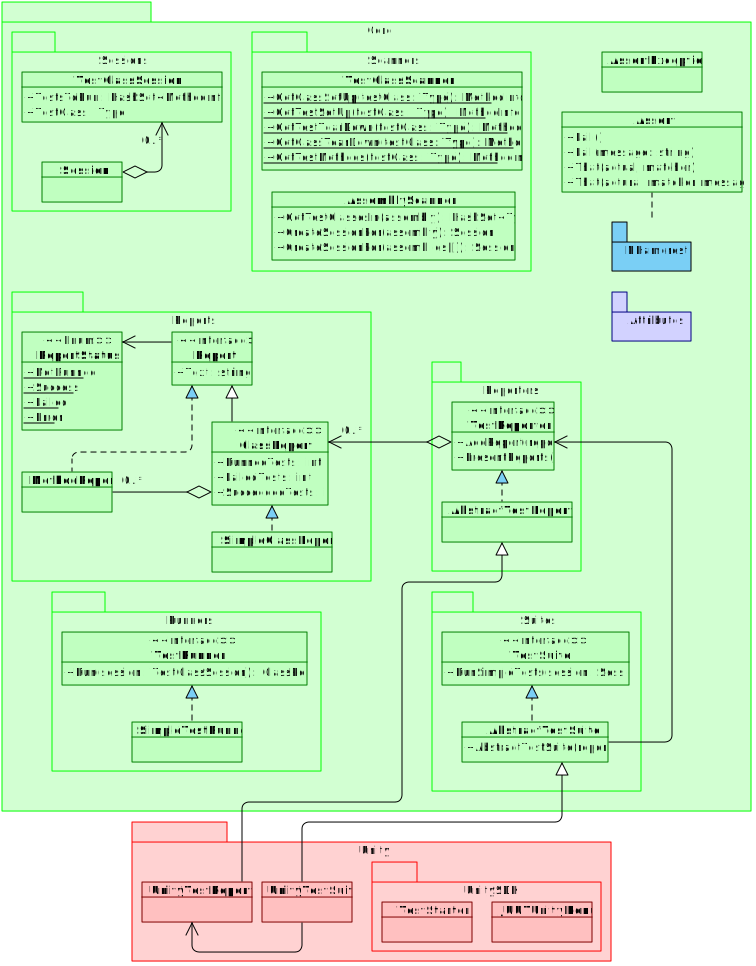
\includegraphics[width=0.9\linewidth]{images/Kapitel_Ergebnis/Overview}
\caption[Übersichtliches Klassendiagramm von JUUT]{Übersichtliches Klassendiagramm von JUUT\\
In diesem Diagramm sind alle Klassen enthalten. Zwecks Übersicht werden nur die wichtigsten Methoden und Attribute dargestellt, sodass man einen Überblick über die Struktur erhält.}
\label{fig:Overview}
\end{figure}
\clearpage

\section{Kernel}

Der Kernel unterteilt sich in mehrere Pakete, welche zu einem bestimmten Aufgabenbereich gehören. Lediglich die Klassen \textit{Assert}, \textit{AssertException} und eine Util-Klasse (welche nicht im Übersichtsdiagramm aufgeführt ist) sind in keinem eigenen Paket.

Die drei Hauptaufgaben des Kernels sind
\begin{itemize}
\item \textbf{Definieren von Tests}\\
Hierfür ist hauptsächlich das Paket \textit{Attributes} zuständig, welches dem Benutzer Attribute zur Verfügung stellt um seine Tests zu markieren. Dazu kommt noch die Klasse \textit{Assert} in Zusammenhang mit der Bibliothek NHamcrest.
\item \textbf{Ausführen der Tests}\\
Die Pakete \textit{Sessions}, \textit{Runners} und \textit{Suites} erfüllen diese Aufgabe, wobei die \textit{Scanner} zu Hilfe genommen werden.
\item \textbf{Präsentation der Testergebnisse}\\
Dies wird von den Paketen \textit{Reports} und \textit{Reporters} durchgeführt. Zusätzlich wird die Klasse \textit{AssertException} verwendet, um den Status eines Testergebnisses zu bestimmen und den Text einer fehlgeschlagenen Bedingung zu formatieren.
\end{itemize}

Wie diese Aufgaben implementiert wurden, möchte ich in den nächsten Abschnitten erläutern.

\subsection{Definieren von Tests}

Zur Definition von Tests stehen dem Benutzer einige Attribute zur Verfügen, mit denen er zum Beispiel Testklassen und Testmethoden markieren kann. Ein ausführliches Klassendiagramm aller Attribute befindet sich auf der nächsten Seite.

Einige der Attributsklassen sind abstrakt und dienen der internen Strukturierung, was für die in späteren Abschnitten erläuterten \textit{Runner} und \textit{Scanner} benötigt wird. Die Wurzel der Hierarchie bildet die abstrakte Klasse \textit{JUUTAttribute} die definiert, dass jedes Attribut einen Namen haben muss, welcher zur Präsentation der Testergebnisse verwendet wird. Außerdem bietet sie eine statische Methode, welche überprüft ob ein beliebiger \textit{Member} (zum Beispiel eine Klasse oder eine Methode) zulässig für das Attribut ist. Deswegen muss jedes nicht-abstrakte Attribut die Methode \textit{Validate} implementieren. Zum Beispiel wird bei einfachen Testmethoden (markiert durch \textit{SimpleTestMethod}) geprüft, dass der Member eine Methode ist und keine Parameter erwartet (s. \autoref{code:SimpleTestMethodAttribute_Validate} \nameref{code:SimpleTestMethodAttribute_Validate}). Hat er allerdings Parameter, wird eine Exception geworfen, um dem Anwender diesen Fehler bei der Präsentation der Testergebnisse mitzuteilen.

\begin{figure}[h]
\centering
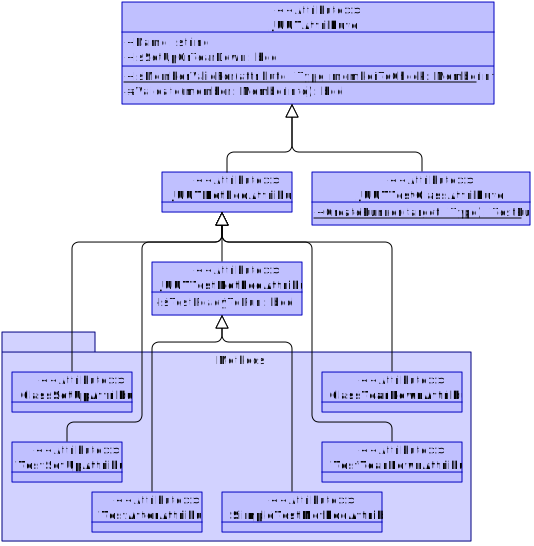
\includegraphics[width=0.9\linewidth]{images/Kapitel_Ergebnis/Attributes}
\caption[Attribute zur Markierung testspezifischer Elemente]{Attribute zur Markierung testspezifischer Elemente}
\label{fig:Attributes}
\end{figure}

Das \textit{JUUTTestClass}-Attribut wir zur Markierung von Testklassen benutzt. Zusätzlich zu den geerbten Funktionalitäten, kann es auch den optimalen \textit{TestRunner} für die markierter Testklasse liefern. Denn je nachdem welche Arten von Tests diese enthält wird ein anderer Typ \textit{Runner} zur fehlerfreien Ausführung benötigt.

Als abstrakte Superklasse aller Testmethoden dient \textit{JUUTTestMethodAttribute}. Dadurch kann einem der \textit{TestClassScanner} alle Tests einer Testklasse liefern, ohne alle konkreten Test-Attribute zu kennen. Es hat ein öffentlich lesbares Attribut \textit{IsReadyToRun} welches angibt, ob der markiert Test schon ausgeführt werden darf. Dies soll von den \textit{Runnern} berücksichtigt werden, wodurch komplexere Testmethoden möglich sind. Für konkrete Tests gibt es die Attribute \textit{SimpleTestMethod} und \textit{TestAfter}. Mit Ersterem markiert man einfache Tests, die immer bereit zur Ausführung sind. Diese sind äquivalent zu den Tests die mit UUnit oder SharpUnit möglich sind. Mit \textit{TestAfter} versehene Tests sollen nach der Ausführung einer bestimmten Methode einer Klasse durchgeführt werden (zum Beispiel die \textit{Update}-Methode eines Skripts). Ursprünglich hatte ich vor diese Funktionalität mit aspektorientierter Programmierung\footnote{Mit AOP lassen sich eigene Funktionalitäten an bestimmte Stellen des Programms einweben. Mehr dazu findet man zum Beispiel in \textit{"`Aspect-oriented programming"} unter anderem von Gregor Kiczales.} zu implementieren. Das Attribut wäre dabei der \textit{Advice} der nach dem Methodenaufruf eingewoben werden würde und einen \textit{ReadyToRun}-Flag auf wahr setzt, wodurch der \textit{Runner} den Test beim nächsten Durchgang ausführt. Allerdings wird zum Umweben einer nicht statischen Methode einer Klasse ein \textit{Proxy-Objekt} benötigt, welches an Stelle des eigentlichen Objekts verwendet wird. Leider ist es nicht möglich in einer laufenden Unity-Umgebung ein Skript durch ein entsprechendes \textit{Proxy-Objekt} zu ersetzen. Zum Zeitpunkt der Fertigstellung dieser Studienarbeit war es mir nicht möglich dieses Problem zu lösen, sodass diese Funktionalität nur schematisch vorhanden ist.

Neben Attributen für Testmethoden, gibt es noch weitere für \textit{SetUp}- und \textit{TearDown}- Methoden. In Sachen definieren von Tests entspricht JUUT also dem Funktionsumfang von MSTest.

Abgesehen von den Attributen sind für Tests noch die möglichen Assertions wichtig. Diese werden von der Klasse \textit{Assert} zur Verfügung gestellt. Durch die Verwendung von
\begin{wrapfigure}{r}{0.5\linewidth}
\centering
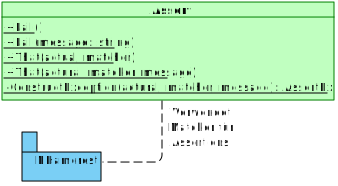
\includegraphics[width=0.95\linewidth]{images/Kapitel_Ergebnis/Assert}
\caption[\textit{Assert}-Klasse von JUUT]{\textit{Assert}-Klasse von JUUT}
\label{fig:Assert}
\end{wrapfigure}
NHamcrest ist diese sehr schlank und bietet dennoch mehr Bedingungen, auf die getestet werden können, als die Standard-\textit{Assert}-Klassen von UUnit, SharpUnit oder MSTest. So werden nur zwei Methoden benötigt. Zum einen die Methode \textit{Fail}, die den Test gezielt fehlschlagen lässt, indem sie eine \textit{AsserException} wirft. Optional lässt sich diese mit einer Nachricht versehen, welche bei der Präsentation angezeigt wird. Dazu kommt noch die Methode \textit{That}. Diese erwartet das zu überprüfende Objekt \textit{actual} und einen \textit{Matcher}, der überprüft ob dieses eine bestimmte Bedingung erfüllt. Bedingungen können sein, dass \textit{actual} nicht Null ist oder dass von einer Anweisung eine Exception geworfen wird.

Abschließend wird gezeigt, wie ein Test mit JUUT definiert werden kann:
\begin{lstlisting}[caption={[Beispiel für einen Test mit JUUT]Beispiel für einen Test mit JUUT\\In diesem Fall sind \textit{Throws.An} und \textit{Is.NotNull} die Matcher, welche den ersten Parameter darauf überprüfen, dass eine Exception geworfen wird beziehungsweise das Objekt nicht Null ist.}, label=code:SimpleTestMethodAttribute_Validate]
[JUUTTestClass]
public class TestClass {
	
	private ClassToTest objectToTest;
	
	[TestSetUp]
	public void SetUp() {
		objectToTest = new ClassToTest();
	}
	
	[SimpleTestMethod]
	public void TestObjectCreation() {
		Assert.That(() => { new ClassToTest(null); }, Throws.An<ArgumentException>());
		Assert.That(objectToTest.ImportantProperty, Is.NotNull());
	}
		
	[TestSetUp]
	public void SetUp() {
		objectToTest = null;
	}
	
}
\end{lstlisting}
\clearpage

\subsection{Ausführen der Tests}

Das Ausführen der Tests ist die Kernfunktionalität eines Test-Frameworks und wird bei JUUT von den Paketen \textit{Sessions}, \textit{Runners} und \textit{Suites}, unter der Zuhilfenahme der \textit{Scanner}, durchgeführt. Die \textit{Sessions} verwalten die auszuführenden Tests, während \textit{Runner} und die \textit{Suite} für das tatsächliche Testen zuständig sind.

Als erstes muss der Anwender mit \textit{Session}-Objekten definieren, welche Tests durchgeführt werden sollen, weswegen dieses Paket zuerst vorgestellt wird.

\begin{figure}[h]
\centering
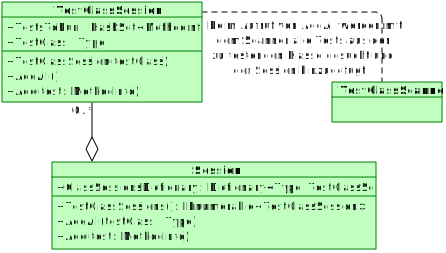
\includegraphics[width=0.8\linewidth]{images/Kapitel_Ergebnis/Sessions}
\caption[\textit{Sessions}-Paket]{\textit{Sessions}-Paket}
\label{fig:Sessions}
\end{figure}

Eine \textit{TestClassSession} repräsentiert eine Testklasse und verwaltet die zu dieser Klasse gehörenden Testmethoden. Sie muss einer mit dem \textit{JUUTTestClass}-Attribut versehenen Klasse zugeordnet werden, weswegen sie als Konstruktor-Parameter einen Typ erwartet. Mit den Methoden \textit{AddAll} und \textit{Add} können alle oder einzelne Testmethoden der Testklasse hinzugefügt werden. Beim Aufruf von \textit{AddAll} durchsucht die statische Hilfsklasse \textit{TestClassScanner} den zugeordneten Typ nach Methoden, welche mit einem \textit{JUUTTestMethod}-Attribut markiert wurden, die dann zur \textit{Session} hinzugefügt werden. Wie das Scannen genau implementiert wurde, sieht man in der Sektion \ref{sec:Appendix_Scanners} \nameref{sec:Appendix_Scanners} im Appendix.

\textit{TestClassSession} dient der JUUT-internen Verwaltung. Vom Anwender muss lediglich eine \textit{Session} erzeugt werden, welche wiederum eine Menge von \textit{TestClassSessions} verwaltet. Diese werden in Form einer Hashtabelle gespeichert, wobei der Schlüssel der Typ der Testklasse und das Element die dazugehörige \textit{TestClassSession} ist. Die Methoden \textit{AddAll} und \textit{Add} von \textit{Session} überprüfen nun, ob es schon eine \textit{TestClassSession} für den hinzuzufügenden Test gibt, erstellen gegebenenfalls eine Instanz und delegieren das Hinzufügen des Tests an das \textit{TestClassSession}-Objekt. Die Definition einer \textit{Session} könnte wie folgt aussehen:
\begin{lstlisting}[caption={[Beispiel für die Definition einer \textit{Session}]Beispiel für die Definition einer \textit{Session}}, label=code:Example_SessionCreation]
Session session = new Session();
session.AddAll(typeof(TestClass));
session.Add(typeof(AnotherTestClass).GetMethod("ATestMethod"));
\end{lstlisting}

Nachdem eine \textit{Session} definiert wurde, müssen die darin enthaltenen Tests ausgeführt werden. Diese Aufgabe übernimmt die \textit{TestSuite} und weitere Klassen, welche im nachfolgenden Klassendiagramm dargestellt sind.

\begin{figure}[h]
\centering
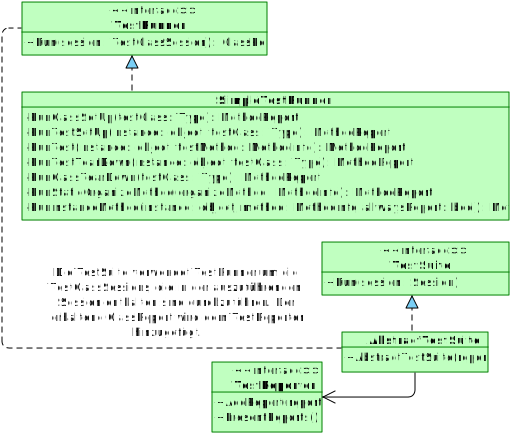
\includegraphics[width=0.8\linewidth]{images/Kapitel_Ergebnis/SuitesAndRunners}
\caption[Für die Ausführung von Tests verantwortliche Klassen]{Für die Ausführung von Tests verantwortliche Klassen}
\label{fig:SuitesAndRunners}
\end{figure}

Eigentlich führen die \textit{TestRunner} die Tests durch, da die \textit{TestSuite} für jede in der \textit{Session} enthaltene \textit{TestClassSession} an einen \textit{TestRunner} delegiert. Der vom \textit{Runner} zurückgegebene \textit{ClassReport} wird dem \textit{TestReporter} hinzugefügt und nach Abschluss wird dessen \textit{PresentReports}-Methode aufgerufen um die Ergebnisse darzustellen.

Der Ablauf innerhalb des \textit{TestRunners} ist wie folgt:
\begin{enumerate}
\item Erzeugung einer \textit{ClassReport}-Instanz
\item Aufruf der \textit{ClassSetUp}-Methode
\item Erzeugung einer Instanz der zu testenden Klasse
\item Für jeden Test der \textit{TestClassSession}
	\begin{enumerate}[label*=\arabic*.]
	\item Aufruf der \textit{TestSetUp}-Methode
	\item Aufruf der Testmethode
	\item Aufruf der \textit{TestTearDown}-Methode
	\end{enumerate}
\item Aufruf der \textit{ClassTearDown}-Methode
\item Rückgabe des gefüllten \textit{ClassReports}
\end{enumerate}

Die einzelnen Methodenaufrufe werden mit Hilfe von \textit{Reflection} durchgeführt. Falls dabei eine Exception geworfen wird, wird diese gefangen und daraus ein \textit{MethodReport} erzeugt, welcher der \textit{ClassReport}-Instanz hinzugefügt wird. Tritt ein Fehler in einer der organisierenden Methoden (z.B. \textit{TestSetUp} oder \textit{TestTearDown}) auf, wird der Durchlauf abgebrochen und der Bericht sofort zurückgegeben, da der Fehler bei jeder einzelnen Testmethode auftreten würde. Die konkrete Implementierung findet man in der Sektion \ref{sec:Appendix_Runners} \nameref{sec:Appendix_Runners} im Appendix.

Eine \textit{Session} lässt sich nun mit folgendem Code ausführen:
\begin{lstlisting}[caption={[Beispiel für die Ausführung einer \textit{Session}]Beispiel für die Ausführung einer \textit{Session}\\\textit{ConcreteTestSuite} ist stellvertretend für eine beliebige Implementierung von \textit{AbstractTestSuite}.}, label=code:Example_SessionCreation]
Session session = new Session();
session.AddAll(typeof(TestClass));
session.Add(typeof(AnotherTestClass).GetMethod("ATestMethod"));

TestSuite suite = new ConcreteTestSuite();
suite.Run(session);
\end{lstlisting}
\clearpage

\subsection{Präsentation der Testergebnisse}

Nachdem die Tests durchgeführt wurden, müssen die Ergebnisse nur noch dem Benutzer präsentiert werden. Da die Form der Präsentation abhängig von der Spiele-Engine ist, worauf in \autoref{sec:Ergebnis_Unity} näher eingegangen wird, beschäftigt sich dieser Teil mit der Strukturierung und Verwaltung der einzelnen Berichte.

~

\begin{figure}[h]
\centering
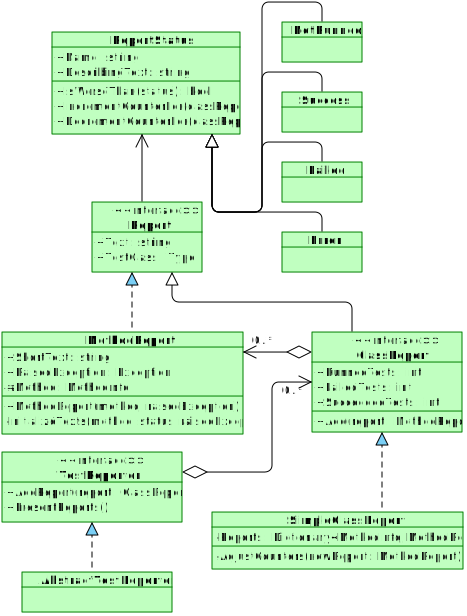
\includegraphics[width=0.8\linewidth]{images/Kapitel_Ergebnis/ReportersAndReports}
\caption[Für die Präsentation der Testergebnisse verantwortliche Klassen]{Für die Präsentation der Testergebnisse verantwortliche Klassen}
\label{fig:ReportersAndReports}
\end{figure}
\clearpage

Das kleinste Teil der Reporting-Maschinerie ist der \textit{ReportStatus}, der die Art des Berichts festlegt. Es gibt die Status \textit{NotRunned}, \textit{Success}, \textit{Failed} und \textit{Error}, wobei der Unterschied zwischen \textit{Failed} und \textit{Error} darin liegt, dass bei Berichten mit dem Status \textit{Error} eine Exception geworfen wurde, die nicht vom Typ \textit{AssertException} ist. \textit{Create} von \textit{ReportStatus} ist eine Fabrikmethode, welche einen zu einer Exception passenden Status erzeugt.

Alle Berichte implementieren dass \textit{Report}-Interface, welches definiert, dass Berichte einen Status und einen Text haben der eine Zusammenfassung des Testdurchlaufs darstellt, sowie einem festen Typ zugeordnet sind. Es gibt zwei unterschiedliche Arten von Berichten. Zum einen \textit{MethodReports}, die den Verlauf einer testspezifischen Methode speichert. Diese haben zusätzlich noch eine Kurzfassung des Verlaufs, eine Referenz auf die geworfene Exception und auf die ausgeführte Methode. Der Text eines \textit{MethodReports} ist abhängig von der geworfenen Exception:
\begin{itemize}
\item Keine Exception\\
\textit{"The Foo-Method passed successfully."}
\item Eine \textit{AssertException}\\
\textit{"The Foo-Method failed: Expected is 10, but was 12."}
\item Keine Exception\\
\textit{"The Foo-Method threw an unexpected exception: Exception-Message"}
\end{itemize}
Bei der Kurzfassung ist die Nachricht der geworfenen Exception nicht vorhanden. Die genaue Erzeugung der Texte sieht man in \autoref{code:MethodReport_InitializeTexts} \nameref{code:MethodReport_InitializeTexts} des Appendix.

Die zweite Art von Berichten (\textit{ClassReport}) sammelt alle \textit{MethodReports} einer Testklasse. Als zusätzliche Informationen bietet sie die Anzahl der durchgeführten, fehlgeschlagenen und erfolgreichen Tests. Der Text besteht aus diesen Zusatzinformationen und der durch Leerzeilen getrennten Kurzfassungen aller enthaltenen \textit{MethodReports}. Der Status eines \textit{ClassReports} ist der schlechteste Status der enthaltenen Methoden-Berichte. Dieser wird mit Hilfe der \textit{IsWorseThan}-Methode des \textit{ReportStatus}  bestimmt.

Der \textit{TestReporter} wiederum sammelt eine Menge von \textit{ClassReports}. Wie diese dann dem Anwender präsentiert werden, hängt von der konkreten Implementierung ab, welche im nächsten Abschnitt beschrieben wird.

\section{Unity}
\label{sec:Ergebnis_Unity}

Im Unity-spezifischen Teil von JUUT sind die Klassen enthalten, mit denen der Anwender arbeiten wird. Diese sind unterteilt in eine Bibliothek, die unter anderem
\begin{wrapfigure}{r}{0.5\linewidth}
\centering
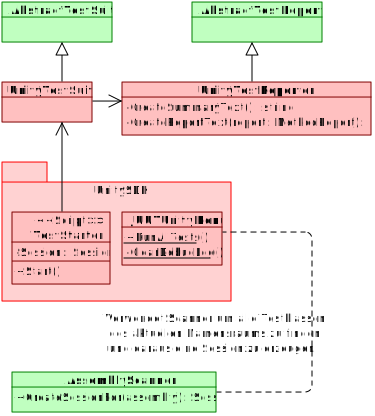
\includegraphics[width=0.95\linewidth]{images/Kapitel_Ergebnis/Unity}
\caption[Unity-spezifische Klassen von JUUT]{Unity-spezifische Klassen von JUUT}
\label{fig:Unity}
\end{wrapfigure}
einen \textit{TestReporter} für Unity enthält und in das Projekt eingebunden werden muss, sowie zwei Klassen, welche als Quelltext vorliegen müssen.

\textit{UnityTestSuite} ist eine konkrete Implementierung von \textit{AbstractTestSuite} und verwendet als Reporter eine Instanz von \textit{UnityTestReporter}, um die Ergebnisse zu präsentieren. Deren Präsentation erfolgt wie bei UUnit oder SharpUnit über die Debug-Konsole von Unity, da es aus Zeitgründen nicht möglich war eine besser Darstellung (wie sie im Ausblick beschrieben wird) zu implementieren. Dabei wird zunächst die Anzahl der ausgeführten und fehlgeschlagenen Tests ausgegeben, gefolgt von einer Liste mit detaillierten Informationen der fehlgeschlagenen Tests. Diese enthalten den \textit{Text} des jeweiligen \textit{MethodReports} und den Stacktrace der geworfenen Exception. Die Präsentation der Testergebnisse sieht zum Beispiel wie folgt aus:
\begin{figure}[h]
\centering
\includegraphics[width=0.9\linewidth]{images/Kapitel_Ergebnis/JUUTTestergebnisse}
\caption[Präsentation der Testergebnisse in Unity]{Präsentation der Testergebnisse in Unity}
\label{fig:JUUTTestergebnisse}
\end{figure}

\textit{TestStarter} ist das Skript, welches für die Ausführung der Tests zuständig ist und an eine beliebiges \textit{GameObject} angehängt werden muss. Im Gegensatz zu dem \hyperref[code:SharpUnitTestRunner]{entsprechenden Skript} in SharpUnit ist es sehr schlank, da man nur die Session definieren und ausführen muss.\\

\begin{lstlisting}[caption={[\textit{TestStarter}-Skript von JUUT]\textit{TestStarter}-Skript von JUUT}, label=code:TestStarter_JUUT]
public class TestStarter : MonoBehaviour {

	private UnityTestSuite Suite = new UnityTestSuite();
	private Session Session = new Session();
	
	// Use this to set up the test suite
	public void Start () {
		Session.AddAll(typeof(TestSample));
		Suite.Run(Session);
	}
	
}
\end{lstlisting}

Wird die Klasse \textit{JUUTUnityMenu} im Pfad \textit{Assets/Editor/} eines Projekts eingebunden, wird wie bei UUnit ein Eintrag in der Menüleiste der Unity-SDK erzeugt, mit dem man alle im Projekt definierten Tests ausführen kann. Dabei wird der \textit{AssemblyScanner} zu Hilfe genommen, der aus einem Namensraum eine \textit{Session} erzeugen kann.
	\chapter{Fazit}

Zeilen source code
Tests Robustheit, Erweiterbarkeit, Usability
	
	% Anhang
	\clearpage
	\pagenumbering{roman}

	% Abbildungsverzeichnis
	\cleardoublepage
	\phantomsection \label{listoffig}
	\addcontentsline{toc}{chapter}{Abbildungsverzeichnis}
	\listoffigures

	% Quellcodeverzeichnis
	\cleardoublepage
	\phantomsection \label{listoflist}
	\addcontentsline{toc}{chapter}{Listings}
	\lstlistoflistings

	% Literaturverzeichnis
	\cleardoublepage
	\phantomsection \label{listoflit}
	\addcontentsline{toc}{chapter}{Literaturverzeichnis}
	\begin{thebibliography}{---}

\bibitem[FRE10]{FRE10}
  \textsc{Steve Freeman und Nat Pryce}: 
  \textbf{Growing Object-Oriented Software, Guided by Tests}.
  2010, Addison-Wesley Professional
  
\bibitem[FEA04]{FEA04}
  \textsc{Michael Feathers}: 
  \textbf{Working Effectively with Legacy Code}.
2004, Prentice Hall
    
\bibitem[HEN10]{HEN10}
  \textsc{Ryan Henson Creighton}
  \textbf{Unity 3D Game Development by Example: Beginner's Guide}.
  2010, Packt Publishing
      
\bibitem[TDGD13]{TDGD13}
  \textsc{Jonas Goldt und Lennart Hensler}
  \textbf{Test Driven Game Development mit Unity 3D}.
  2013, Studienarbeit DHBW Karlsruhe

\end{thebibliography}



	% Abkürzungsverzeichnis
	% vorher in Konsole folgendes aufrufen: 
	%	makeglossaries makeglossaries dokumentation.acn && makeglossaries dokumentation.glo
	\printglossary[type=\acronymtype]
	
	% Glossar
	\printglossary[style=altlist,title=Glossar]
\end{document}

